\documentclass[twocolumn]{emulateapj}
\usepackage{amsmath}
\usepackage{graphicx}
\usepackage{natbib}
\citestyle{aa}

\begin{document}
\title{The Hydrogen Epoch of Reionization Array Dish: Characterization with Electromagnetic Simulations}
\author{
Ewall-Wice Aaron\altaffilmark{1,2},
Richard Bradley\altaffilmark{3,4},
Abraham Neben\altaffilmark{1,2},
Nipanjana Patra\altaffilmark{5},
Nithyanandan Thyagarajan \altaffilmark{6},
Jacqueline Hewitt\altaffilmark{1,2},
Zaki S. Ali\altaffilmark{5},
Judd Bowman\altaffilmark{6},
Carina Cheng\altaffilmark{5},
David Deboer\altaffilmark{5},
Aaron Parsons\altaffilmark{5},
Mariet Venter\altaffilmark{7}
and others.
}

\altaffiltext{1}{MIT Kavli Institute for Cosmological Physics}
\altaffiltext{2}{MIT Dept. of Physics}
\altaffiltext{3}{National Radio Astronomy Obs., Charlottesville VA}
\altaffiltext{4}{Dept. of Astronomy, U. Virginia, Charlottesville VA}
\altaffiltext{5}{Astronomy Dept. U. California, Berkeley CA}
\altaffiltext{6}{School of Earth and Space Exploration, Arizona State U.,
\altaffiltext{7}{Stellenbosh}
Tempe AZ}
\begin{abstract}
Using electromagnetic simulations, we assess the spectral properties of the antenna element of the Hydrogen Epoch of Reionization Array (HERA) in order to both establish a specification for the degree of spectral structure that is permissible to sufficiently isolate foregrounds and allow a detection of the cosmological 21\,cm signal and verify direct laboratory measurements of the dish characteristics. We find that our simulations are in good agreement with field measurements. Using simulations of foregrounds, we find that the $\approx -40$\,dB response at 60\,ns of the HERA dish is sufficient to isolate the cosmological 21\,cm signal $\approx 0.2$\,$h$Mpc$^{-1}$ at $z\approx 8.5$ and obtain a high signal to noise detection of the power spectrum. This study represents the first time that direct measurements a 21\,cm interferometer design have been translated into its ability to constrain the physics of reionization. 
\end{abstract}
\section{Introduction}
Observations of the redshift 21\,cm radiation neutral hydrogen in the intergalactic medium (IGM) have the potential to illuminate the hitherto unobserved {\it dark ages} and {\it cosmic dawn}, revolutionizing our understanding of the first UV and X-ray sources in the universe and how their properties influenced galactic evolution (see \citet{Furlanetto:2006Review}, \citet{Morales:2010}, and \citet{Pritchard:2012} for reviews). As of now, two major experimental endeavors are underway to make a first detection of the 21\,cm signal with most focusing on the Epoch of Reionization (EoR) in which UV photons from early galaxies transformed the hydrogen in the universe from neutral to ionized. The first involves measuring the sky-averaged global signal and is being pursued by experiments such as EDGES \citep{Bowman:2010}, LEDA \citep{Greenhill:2012}, DARE \citep{Burns:2012}, SciHi \citep{Voytek:2014}, and BIGHORNS \citep{Sokolowski:2015} coming online in their planning stages or taking data. The second attempts to observe spatial  fluctuations in the 21\,cm emission using radio interferometers. As of now, a first generation of interferometry experiments are taking data in an attempt to make a first statistical detection of the power spectrum of 21\,cm brightness temperature fluctuations. These include the Giant Metrewave Telescope (GMRT)  \citep{Paciga:2013}, the Low Frequency ARray (LOFAR), \citep{VanHaarlem:2013}, the Murchison Widefield Array \citep{Tingay:2013} and the Precision Array for Probing the Epoch of Reionization (PAPER) \citep{Parsons:2010}. 

The primary obstacle to obtaining a high redshift detection of the cosmological signal through both of these methods is the existence of foregrounds that are $\sim 10^5-10^6$ times brighter. While requiring much greater sensitivity to global-signal experiments, interferometers have the advantage that these spectrally smooth foregrounds naturally avoid a significant region of $k$-space, known as the {\it EoR window}, occupying a region known as the {\it wedge} \citep{Datta:2010,Vedantham:2012,Parsons:2012,Thyagarajan:2013,Liu:2014a,Liu:2014b}, however any structure in the frequency response of the instrument has the potential to leak foregrounds into the EoR window, masking our signal. Indeed, low level spectral structures in the analogue and digital signal chains on the initial buildout of the MWA are proving to be a significant obstacle \citep{Dillon:2015b,EwallWice:2015a,Beardsley:2015b}. 

While, in principle, spectral structure in the bandpass of the instrument may be removed in calibration, simulations show that any mismodeling of emission and the primary beam, potentially below the confusion limit, will mix the significant spectral structure on long baselines into short ones, masking the signal entirely \citep{Barry:2015}. While redundant calibration \citep{Wieringa:1992,Liu:2011,Zheng:2014} is able to calibrate the independent of a detailed model of the sky, any direction-dependent chromatic structure in the primary beam of the instrument introduces additional degrees of freedom that must be modeled, potentially leading to signal loss and the introduction of spurious spectral structure due to unmodeled foregrounds in long baselines. Because of our limited knowledge of foregrounds at low-frequency and the fidelity of calibration algorithms, the only sure way of building an instrument that will guarantee a detection of the redshifted 21\,cm emission is to design it such that all spectral structure in the signal chain is limited to a finite region of delay space, well below the wedge.


The Hydrogen Epoch of Reionization Array (HERA) is an instrument currently taking first observations in the Karoo in South Africa with the ultimate goal of detecting the power spectrum of 21\,cm brightness temperature fluctuations at high signal-to-noise (SNR) \citep{Pober:2014}. A central principle in HERA's design is that it be calibration fail-safe such that a detection of the signal is guaranteed, even if the chromaticity of the instrument is not calibrated out. This paper and its companions \citep{Neben:2015b,Patra:2015,Thyagarajan:2015c} describe a multifaceted approach to establishing a stringent specification on the spectral structure permissible for HERA to be calibration fail-safe and determine to what extent its design meets these requirements. We accomplish this by establishing a spec with simulations of foregrounds \citep{Thyagarjan:2015c} and verifying that HERA primary antenna element meets this spec with reflectometry \citep{Patra:2015} and Orbcomm beam mapping \citep{Neben:2015b}. These measurements are verified with detailed electromagnetic simulations which we describe in this work. 

This paper is organized as follows. In \S~\ref{sec:Formalism} we lay out our analytic framework for describing the impact of reflections and spectral structure on foreground leakage in delay-transform power spectra. In \S~\ref{sec:Simulations} we describe our electromagnetic simulations of the HERA dish element. In \S~\ref{sec:Comparison} we compare our simulation results to direct measurements of the primary dish element and in \S~\ref{sec:Foregrounds} we apply our electromagnetic simulation results to simulations of foregrounds to determine the extent that the HERA dish's chromatic structure pollutes the EoR window and their impact on HERA's overall sensitivity. We conclude in \S~\ref{sec:Conclusion}.

\section{The Impact of Reflections on Delay-Transform Power Spectra}\label{sec:Formalism}
In this section, we show how reflections in the analogue signal path of an antenna lead to foreground contamination of the EoR window. Intuitively, any reflections in the signal path introduce sinusoidal ripples in the frequency dependent gain of the instrument. Since reflection delay is the Fourier dual to frequency, reflections at larger delays introduce ripples at higher frequencies. Isolation of the 21\,cm signal from foregrounds that are over five orders of magnitude brighter depends critically on their smoothness. Any sinusoidal frequency structure, introduced by the antenna gain will cause these foregrounds to mimic and swamp the signal unless they are brought below a level similar to the ratio between the foregrounds and the signal itself. We now derive this process in formal detail. A simple equation for effect of direction independent reflections in the signal chain of an interferometer, downstream of the receiver, has been derived in \citet{EwallWice:2015a}, we extend this analysis in this section by considering the direction dependent reflections that can occur within the antenna element. We assume that the intensity field on the sky is given by 
\begin{equation}\label{eq:Dirac}
I({\bf \widehat{k}},f) \delta_D({\bf \hat{k}} - {\bf \hat{k}'})= \langle s({\bf \hat{k}},f)s^*({\bf \hat{k}'},f)  \rangle_t^2
\end{equation}
 where $\delta_D$ is the Dirac delta function and $\langle \rangle_t$ indicates an average in time. We imagine that the electric field as a function of time, $\widetilde{s}({\bf \widehat{k}},t)$ arrives at an arbitrary origin at time $t$ and at the various $i^{th}$ antenna elements of an interferometer at locations ${\bf x_i}$ at times $\tau_i={\bf x_i} \cdot {\bf \widehat{k}} /c$. We now consider reflections within a single dish element described by a direction dependent reflection coefficient\footnote{Ignoring reflections between multiple dish elements which we treat in Appendix~\ref{app:Reflections}}, $\widetilde{r}_i({\bf \widehat{k}},\tau)$. which re-introduce the signal at later times $\tau$. The voltage signal measured at the $i^{th}$ antenna element, $\widetilde{v}_i$, is the integral over solid angle of the convolution of the electric field entering the antenna (delayed by $\tau_i$) with $r_i({\bf \widehat{k}},\tau')$.

\begin{equation}
\widetilde{v}_i(t) = \int d \Omega \int d \tau \widetilde{r}_i({\bf \widehat{k}},\tau) \widetilde{s}({\bf \widehat{k}},t- \tau_i - \tau)
\end{equation}

A correlator (FX and XF) measures the time-averaged product of the Fourier transform of the voltage streams between the $i^{th}$ and $j^{th}$ antenna. Fourier transforming the voltage stream from the $i^{th}$ antenna we obtain
\begin{equation}
v_i(f) = \int d \Omega \int d \tau \widetilde{r}_i({\bf \widehat{k}},\tau) s({\bf \widehat{k}},f)e^{-2 \pi i f(\tau_i+\tau)}
\end{equation}
The time averaged product between the two antennas is
\begin{equation}
V_{ij}'(f) = \left \langle v_i(f) v_j^*(f) \right \rangle_t = \int d \Omega \int d \tau \widetilde{r}_i(\tau) d \tau' \widetilde{r}^*_j(\tau')e^{-2 \pi i f (\tau-\tau') } I({\bf \widehat{k}}, f) e^{- 2 \pi i \Delta \tau_{ij}f} 
\end{equation}
where $\Delta \tau_{ij} = \tau_i-\tau_j = ({\bf x_i - x_j}) \cdot {\bf \widehat{k}}/c$. We eliminated one of the solid angle integrals using equation~\ref{eq:Dirac}. 

Defining ${\bf u}_{ij} = f ({\bf x}_i-{\bf x}_j)/c$, we obtain,
 %HERA's primary antenna element consists of a sleeved dipole element suspended 5\,m above the focus of a 14\,m diameter parabolic dish (Fig.~\ref{fig:Dish}).
.
%\begin{figure}
%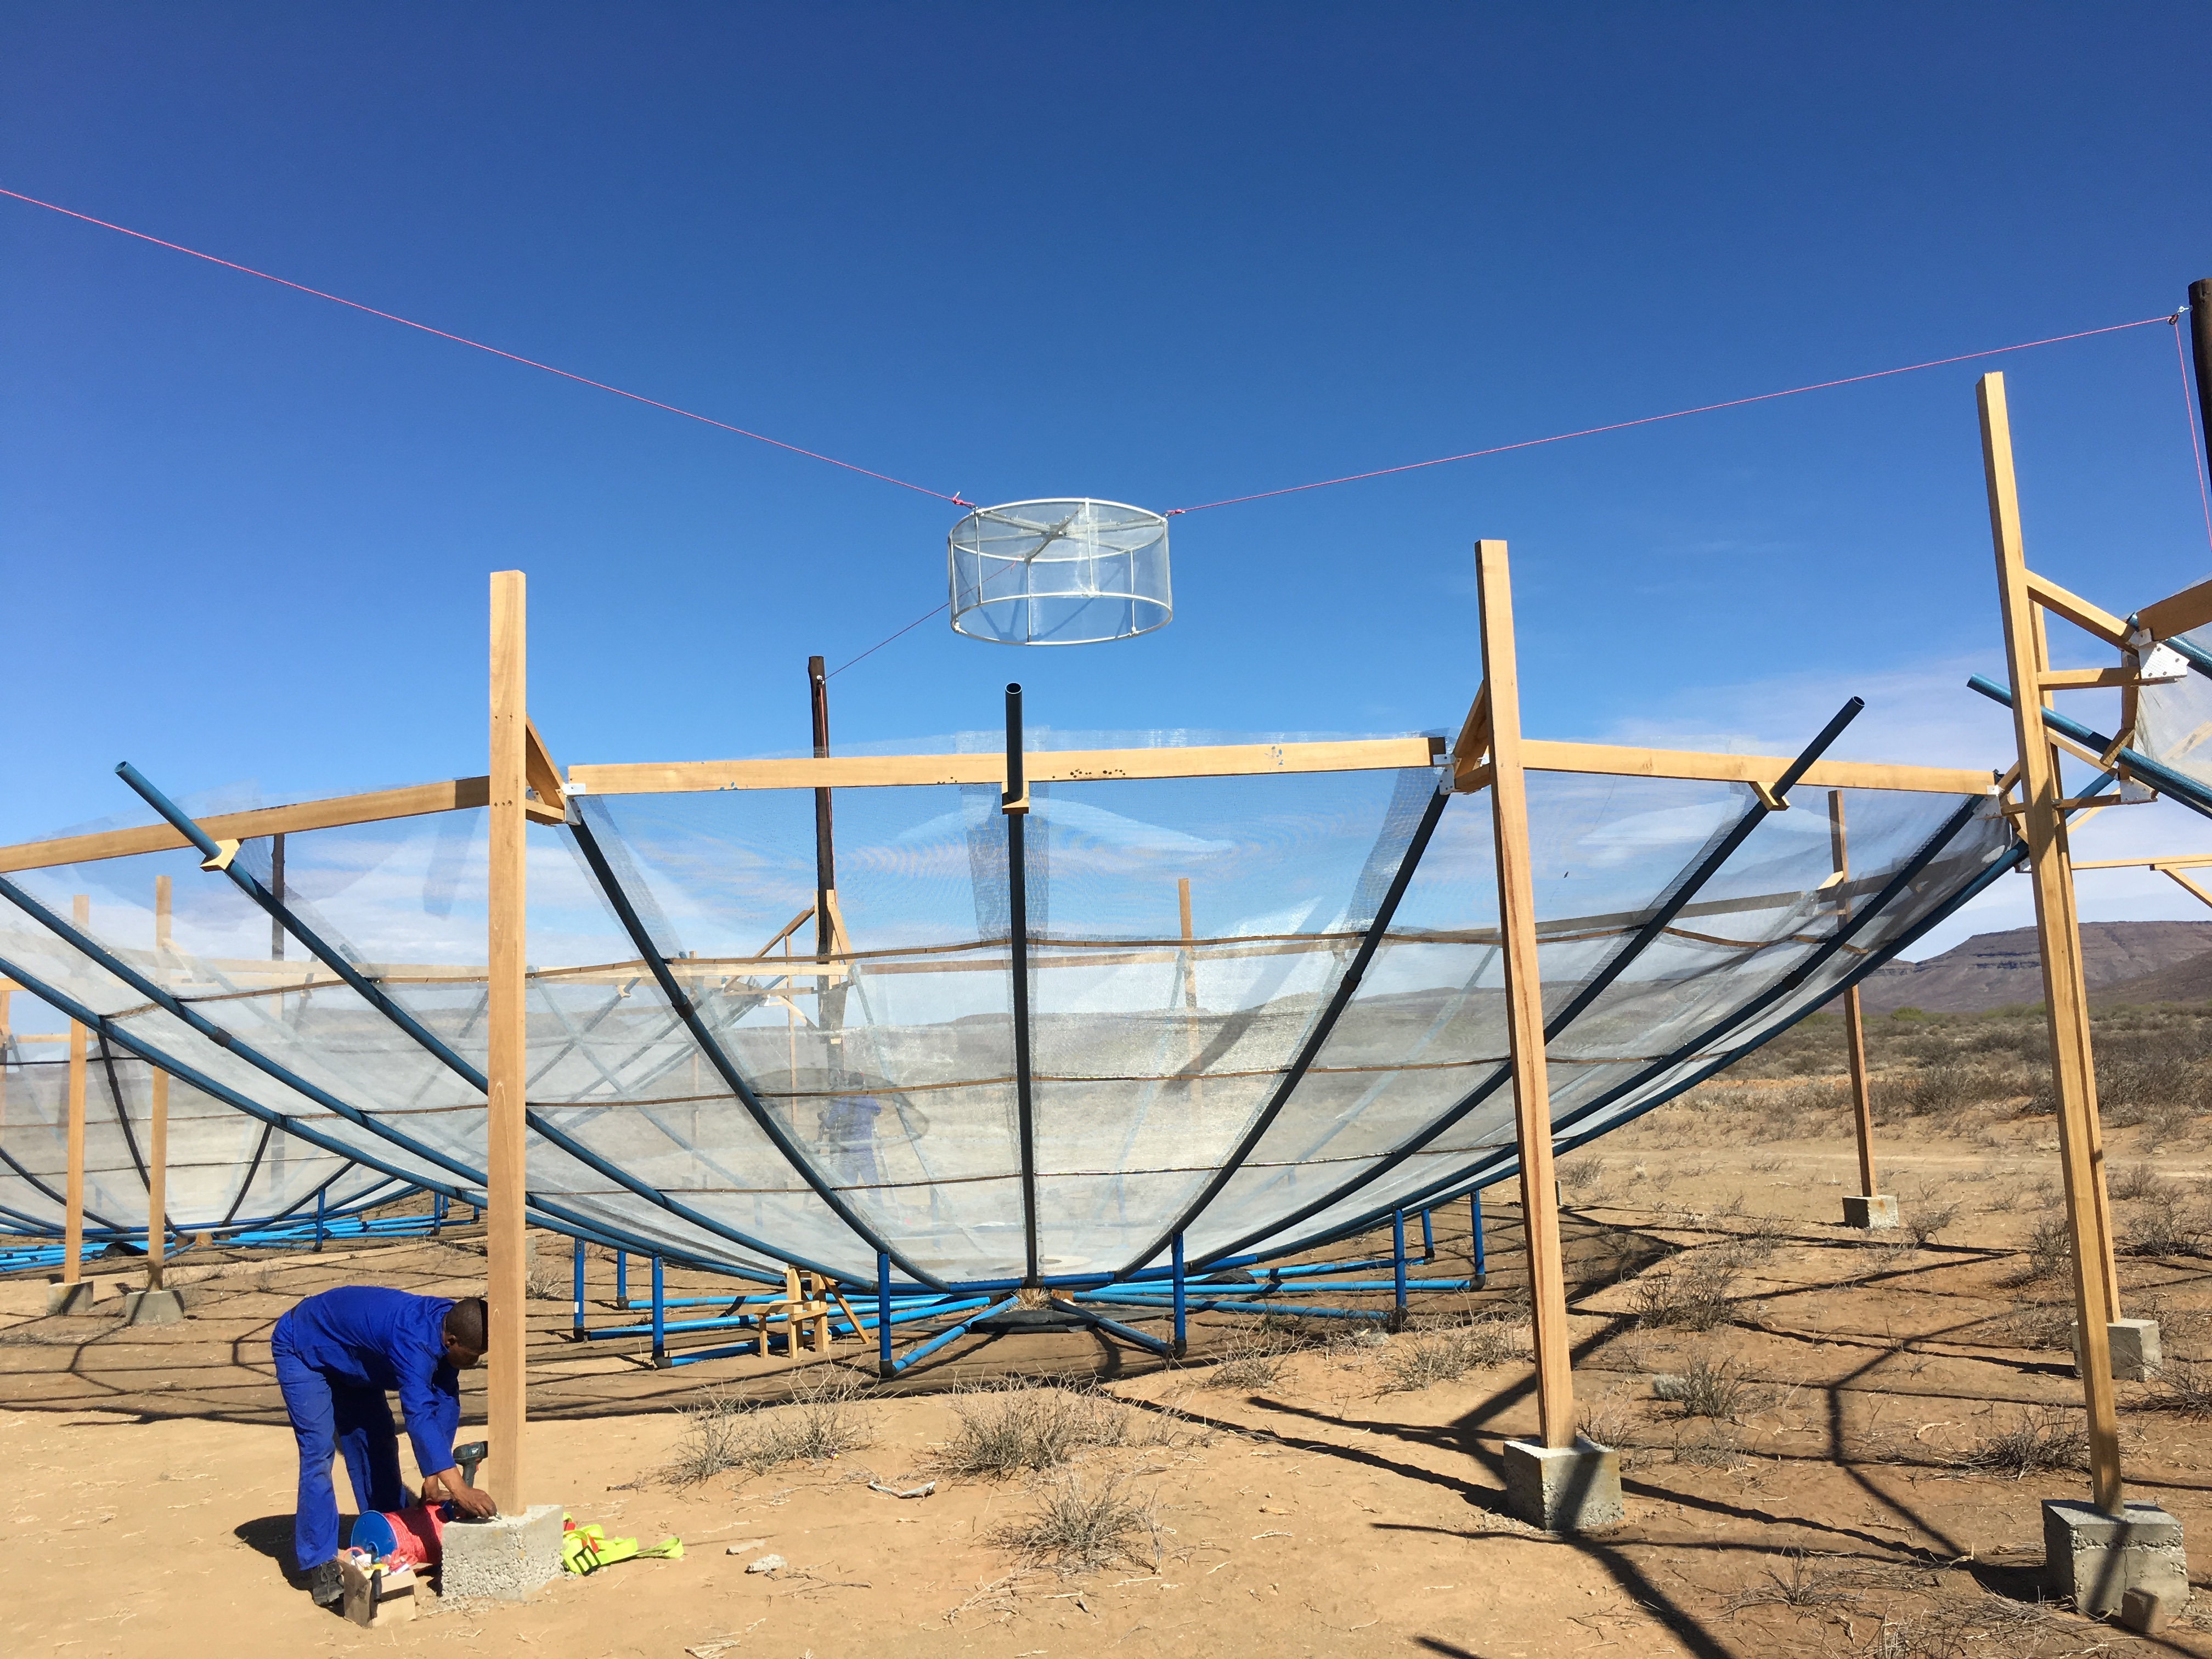
\includegraphics[width=.5\textwidth]{figures/DishSA.png}
%\caption{The HERA primary antenna element-one of 19 undergoing currently taking the first observations in the Karoo in South Africa. The antenna consists of a sleeved dipole suspended within a 2\,m diameter skirt, five meters above the ground at the focal point of a 14\,m diameter dish.}\label{fig:Dish}
%\end{figure}

% We show in Appendix~\ref{app:Reflections} that if an astronomical radio signal with time dependence at the location of the feed, $s({\bf \widehat{k}},t)$, experience reflections within the dish such that the voltage recorded in the feed is 
 
 

Than the resulting visibilities obtained by cross correlating antenna $i$ and antenna $j$ are given by 
\begin{equation}\label{eq:Visibility}
V'_{ij}(f) =  \int d \Omega r_i({\bf \widehat{k}},f) r^*_j({\bf \widehat{k}},f)  I(f,{\bf \widehat{s}})e^{2 \pi i f {\bf u}_{ij} \cdot {\bf \widehat{k}}/c},
\end{equation}
where ${\bf b}_{ij} = ({\bf x}_i - {\bf x}_j )$ to use the usual $uv$ notation of interferometry. $r_i({\bf \hat{k}},f)$ is the inverse fourier transform of the reflection response of the dish, hence we see that the reflection response is precisely the Fourier dual to the Dish's frequency domain voltage beam. Setting a specification on reflections is hence equivalent to setting a specification on the spectral smoothness of the voltage beam. 

In order to separate spectrally smooth foregrounds from our signal, we expect to use the {\it delay transform} over frequency, defined as \citep{Parsons:2012}
\begin{equation}
\widetilde{V}_{ij}(\tau) = \int d f e^{2 \pi i \tau f} V_{ij}(f)
\end{equation}
Applying this to equation~\ref{eq:Visibility}, we obtain
\begin{equation}
\widetilde{V}'_{ij}(\tau)=  \int d \Omega \int d f  r_i({\bf \widehat{k}},f) r_j^*({\bf \widehat{k}},f)  I(f,{\bf \hat{k}}) e^{2 \pi i f ( {\bf b}_{ij} \cdot {\bf \hat{k}} /c - \tau)}
\end{equation}
Let's examine the quantity within the angular integral. For each ${\bf \hat{k}}$, we see that each source is mapped to a line $\tau ={\bf b}_{ij}\cdot{\bf \hat{k}}/c$, resulting in the much discussed ``wedge" \citep{Datta:2010,Vedantham:2012,Parsons:2012,Morales:2013,Thyagarajan:2013,Liu:2014a,Liu:2014b}. The presence of the frequency dependent beam causes each source line to be convolved in delay with the direction dependent kernel
\begin{equation}\label{eq:Kernel}
\widetilde{R}_{ij}({\bf \hat{k}},\tau) = \int d \tau \widetilde{r}_i({\bf \widehat{k}},\tau - \Delta \tau) \widetilde{r}^*_j({\bf \widehat{k}},-\Delta \tau).
\end{equation}
which is the convolution of the delay response of voltage beam $i$ with the complex conjugate of voltage beam $j$ evaluated on a negative t-axis, $\widetilde{r}_i({\bf \widehat{k}},\tau)$,$\widetilde{r}_j({\bf \widehat{k}},\tau)$. Note that this is not equal to the convolution of the voltage response with its complex conjugate, which would lead to foreground power only being bled out to positive delays. Usually, beams have a different delay structure in each direction, and we demonstrate the effect of foreground smearing in Fig.~\ref{fig:Smearing} for a simple model with only three sources. Without reflections, the sources would form lines in $b-\tau$ space. With the reflections, the sources are smeared out, leading to supra-horizon emission. 
\begin{figure*}[h!]
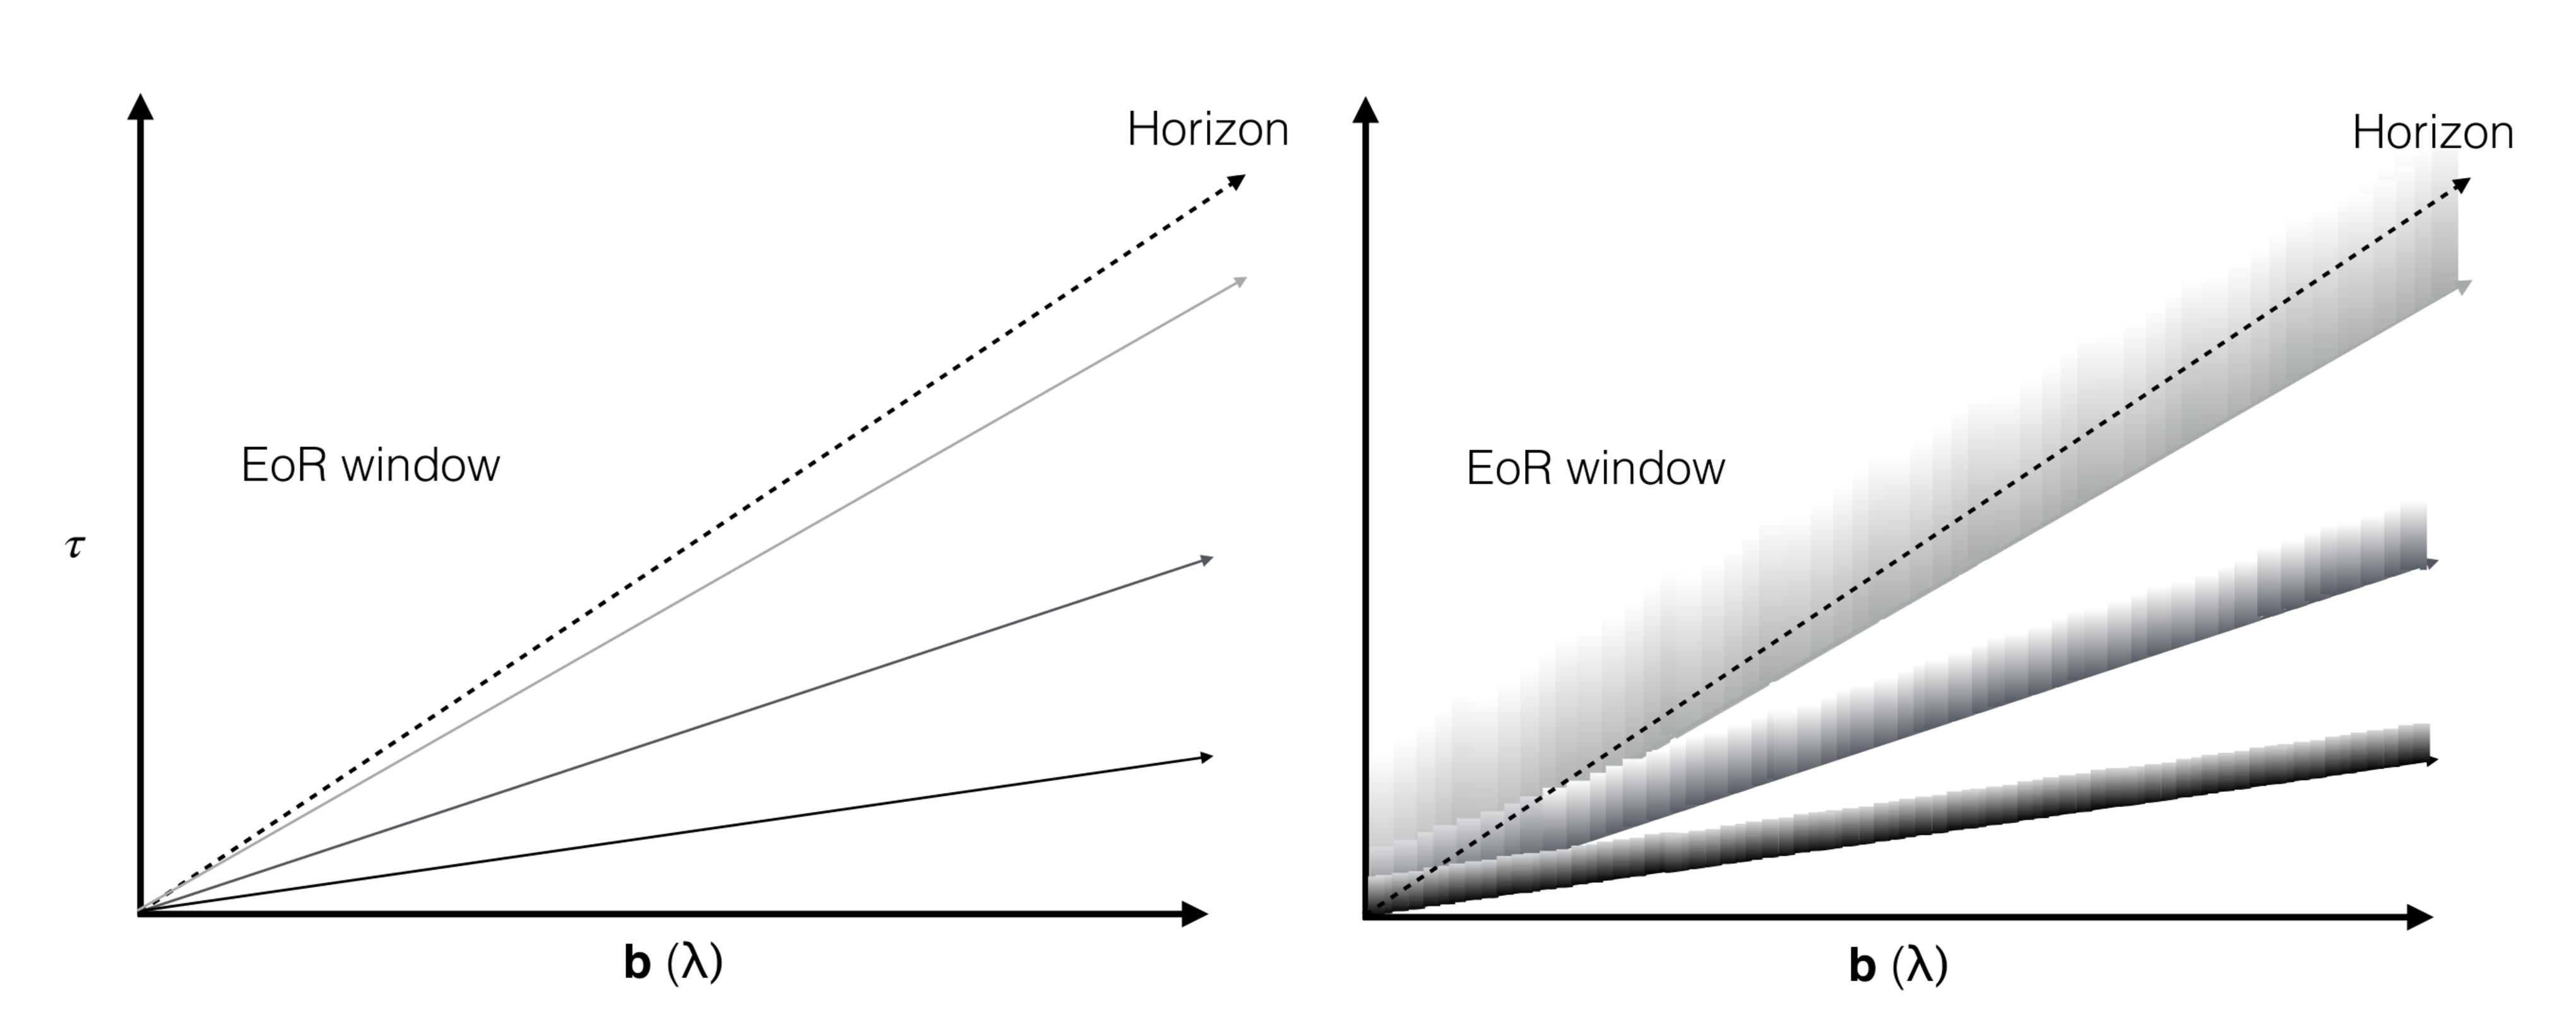
\includegraphics[width=\textwidth]{figures/wedgeCompare.pdf}
\caption{We demonstrate the impact on foregrounds of the frequency dependent beam. Left: The location of three sources in delay space assuming a frequency indepdendent beam (no reflections in the antenna element). Right: the presence of chromaticity due to reflections in the antenna smears the source in delay with the kernel given by equation~\ref{eq:Kernel}. Since the frequency response of the dish are a function of direction on the sky, the shape of the delay kernel is different for each source line. We see that this smearing can lead to substantial supra-horizon emission. Sources near zenith (low delay) tend to have a larger maximum since the beam gain is larger near zenith, but a more compact kernel (since beam bore-sights tend to have less spectral structure). Meanwhile, sources near the horizon have a much smaller maxima but have less compact kernels.}
\label{fig:Smearing}
\end{figure*}
For the sake of pedagogy, we now consider the case where the beam can be factored into angular and frequency dependent components, $r_i({\bf \hat{k}},f) = g_i(f)a_i({\bf \hat{k}})$. For such a case, every line in Fig.~\ref{fig:Smearing} would be convolved with the same delay dependent shape, normalized to the gain of $a_i({\bf \hat{k}})$. In this case, we have
\begin{equation}
\widetilde{V}_{ij}'(\tau) = \int d\tau' \int d \tau'' \widetilde{g}_i(\tau' - \tau'')\widetilde{g}^*_j(\tau'') \widetilde{V}_{ij}(\tau-\tau')
\end{equation}
We can further simplify matters by assuming that $\widetilde{g}_i(\tau=0)\gg\widetilde{g}_i(\tau>0)$, which is often a good assumption at large delays for the relatively smooth bandpasses our instruments are designed to have. 
\begin{equation}\label{eq:KernelApprox}
\widetilde{V}_{ij}'(\tau) \approx \widetilde{g}_i(0)\int d \tau' \widetilde{g}_j^*(\tau')\widetilde{V}_{ij}(\tau- \tau') + \widetilde{g}_j^*(0) \int d \tau' \widetilde{g}_i(\tau')\widetilde{V}_{ij}(\tau-\tau') 
\end{equation}
Hence, to first order, the impact of reflections is to convolve the delay-transformed visibility with the voltage beam of the instrument, which acts as the power-kernel. This may be a somewhat un-intuitive result since we might naively expect for the power-kernel to be the square of the delay-response. This linear falloff puts exquisite requirements on the smoothness of the beam, requiring that it fall roughly six orders of magnitude in delay before the signal is accessible. 


 In this paper, we derive $\widetilde{r}_i({\bf \widehat{k}},\Delta \tau)$ for the HERA antenna element using electromagnetic simulations, in order to verify direct measurements of the antenna element with refelctometry \citep{Patra:2015} and Orbcomm measurements of the beam \citep{Neben:2015b}. We also explore the implications of the HERA dish's $\widetilde{r}_i({\bf \widehat{k}},\tau)$ on the scientific bottom line for EoR, using the Fisher Matrix Formalism. 

\section{Electromagnetic Simulations of the HERA dish element}\label{sec:Simulations}
In Fig.~\ref{fig:SimulationSetup} we show the geometery of the electromagnetic simulation. {\bf Rich: fill in the details here}
\begin{figure}


\subsection{The Simulations}
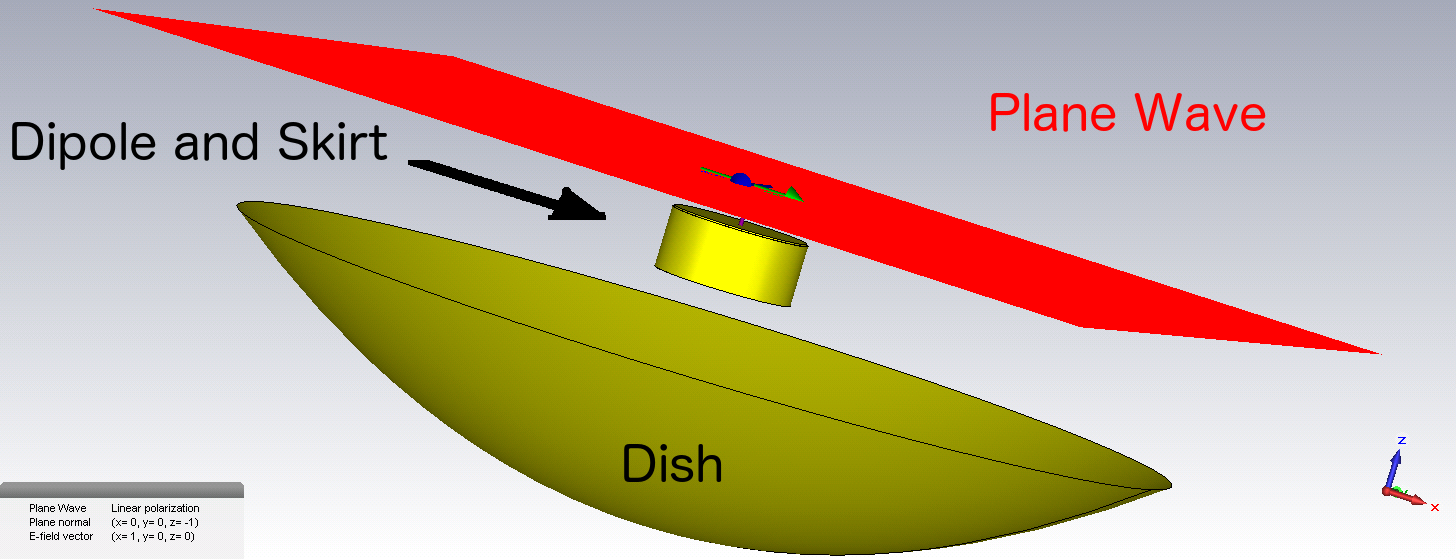
\includegraphics[width=.5\textwidth]{figures/One_dish_Pfeed_render_pw_0deg.png}
\caption{A rendering of our time domain simulation at $t=0$, demonstrating the geometry and setup of our electromagnetic simulation. The plane wave is started just above the feed (red plane).}\label{fig:SimulationSetup}
\end{figure}

\begin{figure*}
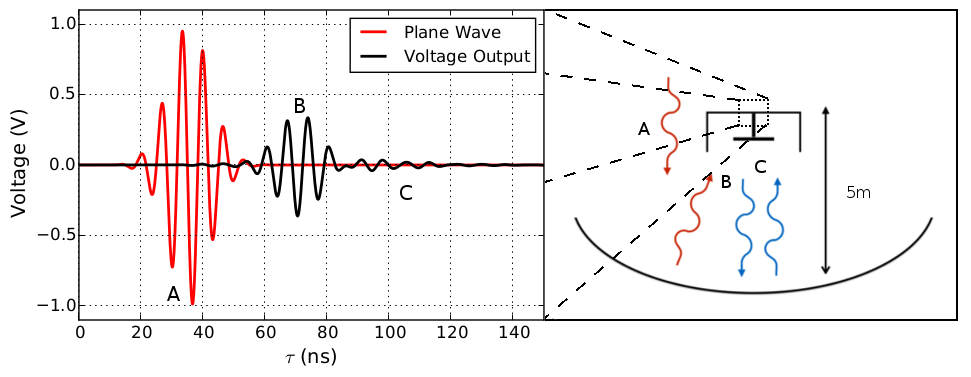
\includegraphics[width=\textwidth]{figures/SimulationIllustration.png}
\caption{An illustration of our simulation products and their origin in the HERA antenna geometry. A plane wave is injected from above the feed (red line). The amplitude of the electric field of the plane wave at output of the feed along with the voltage at the feed terminal outputs is recorded (black line). The feed in our simulation is situated $5$\,m above the bottom of the dish, hence there is a $\approx 30$\,ns delay between when the plane wave passes the terminal for the first time (A) and when it is first absorbed in the dipole (B), leading to the voltage response. Of concern to 21\,cm experiments are the subsequent reflections between the feed and the dish (C) which can lead to large delay contamination of the EoR window.}
\label{fig:Simulation}
\end{figure*}
\subsection{Deconvolving the Response Function}\label{ssec:Deconvolve}
Since our simulation is sampled in finite time steps, we will adopt discretized notation for this section. In particular, our simulation consists of $N$ samples, evenly spaced by $d \tau$ at times $\tau_n = n \times d \tau$. 
In our simulation, we obtain the voltage at the feed output at time $\tau_n$ which we will call $\widetilde{v}_n$. It is related to the input plane wave through the discrete convolution 
\begin{equation}
\widetilde{v}_n({\bf \widehat{k}}) = \sum_m \widetilde{r}_m({\bf \widehat{k}}) \widetilde{s}_{n-m}({\bf \widehat{k}}),
\end{equation}
We may undo this convolution by taking a discrete Fourier transform (DFT) of both ${\bf \widetilde{v}}$ and ${\bf \widetilde{s}}$ in time, dividing them in Fourier space, and taking an inverse DFT back. Symbolically,
\begin{equation}
{\bf \widetilde{r}}({\bf \widehat{k}}) = \boldsymbol{\mathcal{F}}^{-1} \left[ \frac{\boldsymbol{\mathcal{F}} {\bf \widetilde{v}}({\bf \widehat{k}})}{{\bf \widetilde{s}}({\bf \widehat{k}})} \right] 
\end{equation}
where $\boldsymbol{\mathcal{F}}$ is the Fourier transform matrix for a 1d vector of length $N$. 
\begin{equation}
\boldsymbol{\mathcal{F}}_{mn} = e^{2 \pi i m n /N}
\end{equation}
In Fig.~\ref{fig:FrequencyDomain} we show the amplitude of the Fourier transform of our Gaussian input, centered at $150$\,MHz along with the voltage response. Since our input is band limited between $\approx 20$ and $280$\,MHz, the direct ratio of our voltage response and input wave is dominated by numerical noise outside of this range. We eliminate these numerical artifacts by multiplying our ratio by a Blackman-Harris window between $100$\,MHz and $200$\,MHz and set our estimate to zero elsewhere. From a physical standpoint, this is sensible since 21\,cm experiments only observe a limited bandwidth. PAPER's correlator, which will initially serve as the HERA backend samples over a $100$\,MHz instantaneous freqeuency interval. Hence analogue filtering is applied to limit the incoming signal within a finite bandwidth and prevent aliasing.

\begin{figure}[h!]
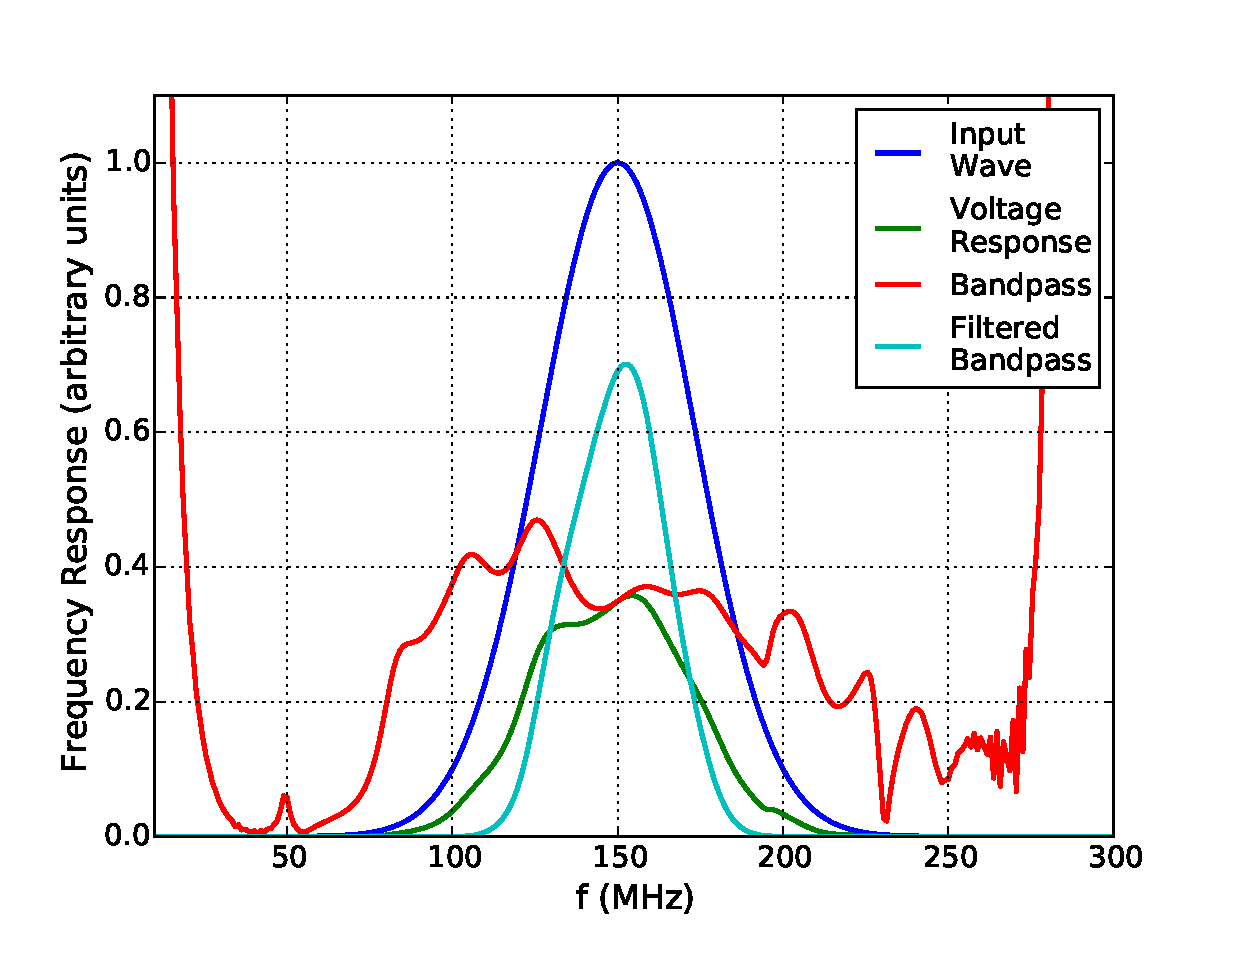
\includegraphics[width=.5\textwidth]{figures/frequency_domain.pdf}
\caption{The absolute value of the discrete Fourier transform of our simulation outputs. We obtain the effective response function of the dish by Fourier transforming the voltage output from our dish (green line) and dividing by the Fourier transform of the input wave (blue line). The simple ratio is plotted as a red line. Since our input is limited to frequencies between $\approx 20$ and $280$\,MHz, there is significant numerical noise that will effect our result outside of this region which we see in the divergene of the red line towards the edges of the plot. To eliminate this noise, we multiply by a Blackman-Harris window between $50$ and $250$\,MHz and set our estimate to zero elsewhere. The Fourier transform of our response estimate with the filter applied is shown as a cyan line.}
\label{fig:FrequencyDomain}
\end{figure}

We plot the delay transform of the voltage response of the dish in Figure~\ref{fig:Simulations} to gauge the dynamic range of our simulations. Since signal at negative delays violates causality, we assume such features are sourced by numerical artifacts such as side-lobes and/or numerical precision noise. We see that our simulations have a dynamic range of $-60$\,dB.


\begin{figure}[h!]
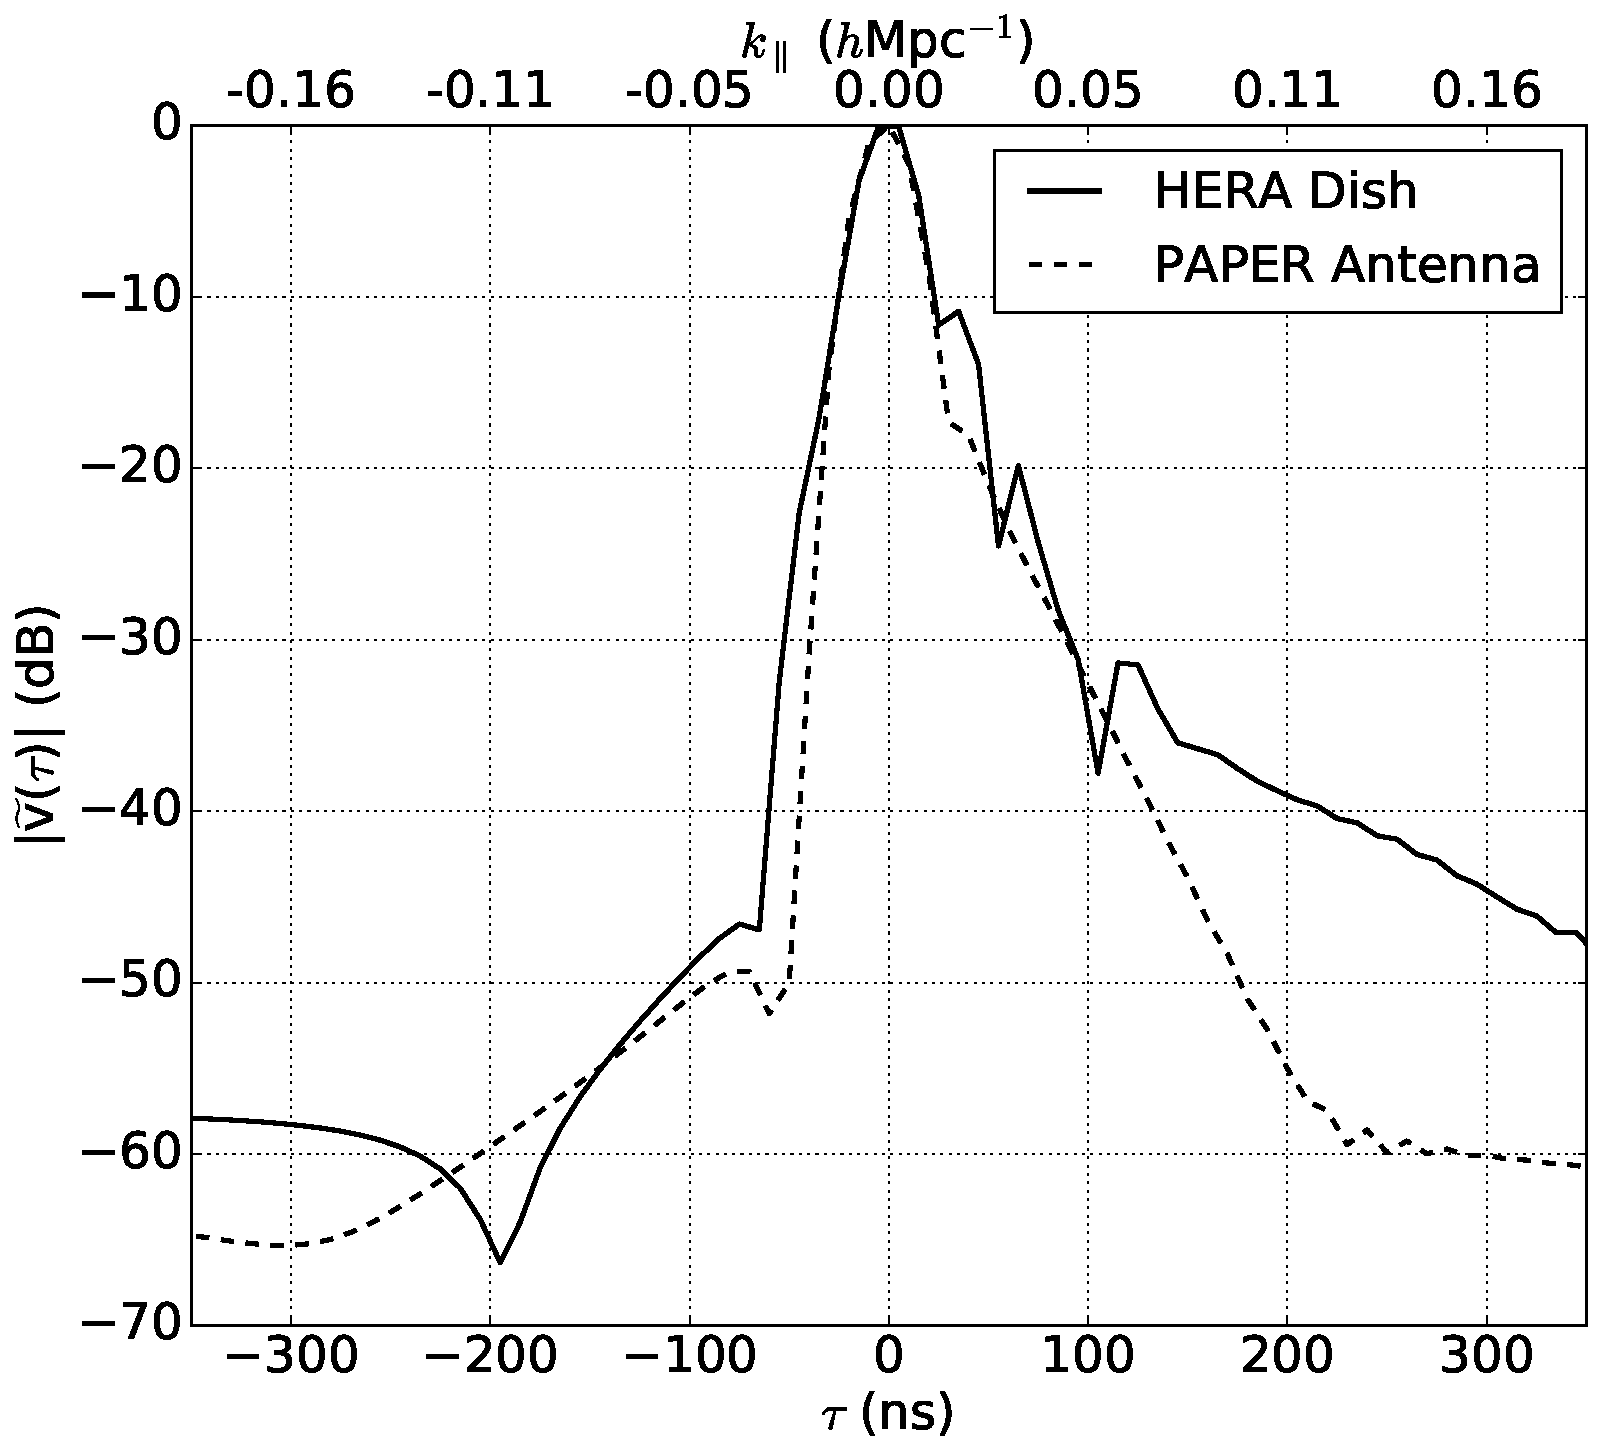
\includegraphics[width=.5\textwidth]{figures/compare_simulations_paper.pdf}
\caption{The Fourier transform of the voltage response function of our simulation for the HERA Dish (solid black line) and the PAPER antenna element (dashed black line). Reflections in the HERA dish element lead to significantly enhanced power above $\sim 50$\,ns. We show the negative delays, which should be devoid of signal, to determine the dynamic range of our technique (which is limited by sidelobes and numerical artifacts). We see that these contaminants exist at the $\sim-60$\,dB level.}
\label{fig:Simulations}
\end{figure}


\begin{figure}
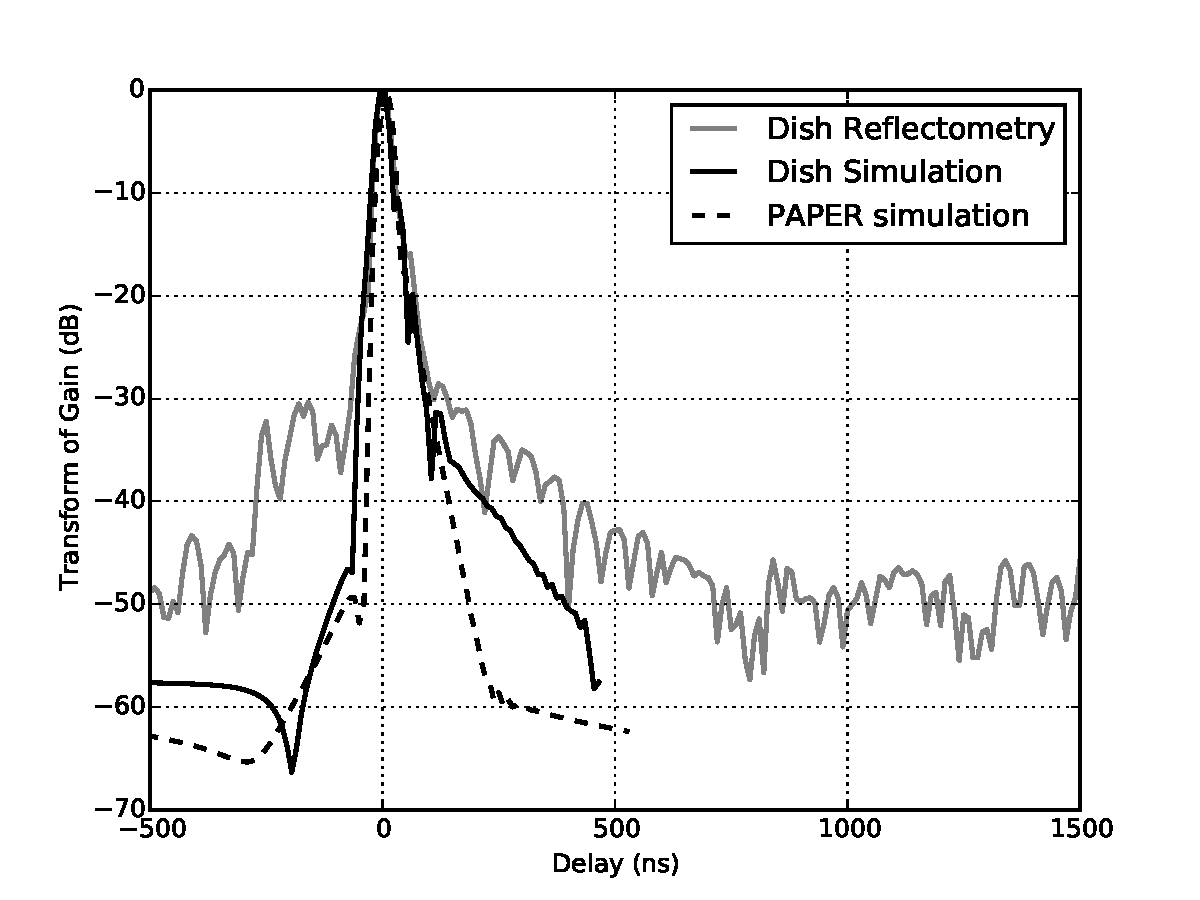
\includegraphics[width=.5\textwidth]{figures/compare_reflectometry_paper.pdf}
\caption{Same as Fig.~\ref{fig:Simulations} but now including 
 the reflectometry measurements of \citep{Patra:2015}. Inspecting negative delays, we see that the reflectometry measurements contain artifacts introduced by reflections and sub-reflections in the cables leading from the VNA to the feed which enter both the HERA dish and PAPER measurements at both the $-45$\,dB to $-30$\,dB level. The VNA measurement is noise dominated beyond $\sim 500$\,ns.}\label{fig:Reflectometry}
\end{figure}

\begin{figure}[h!]
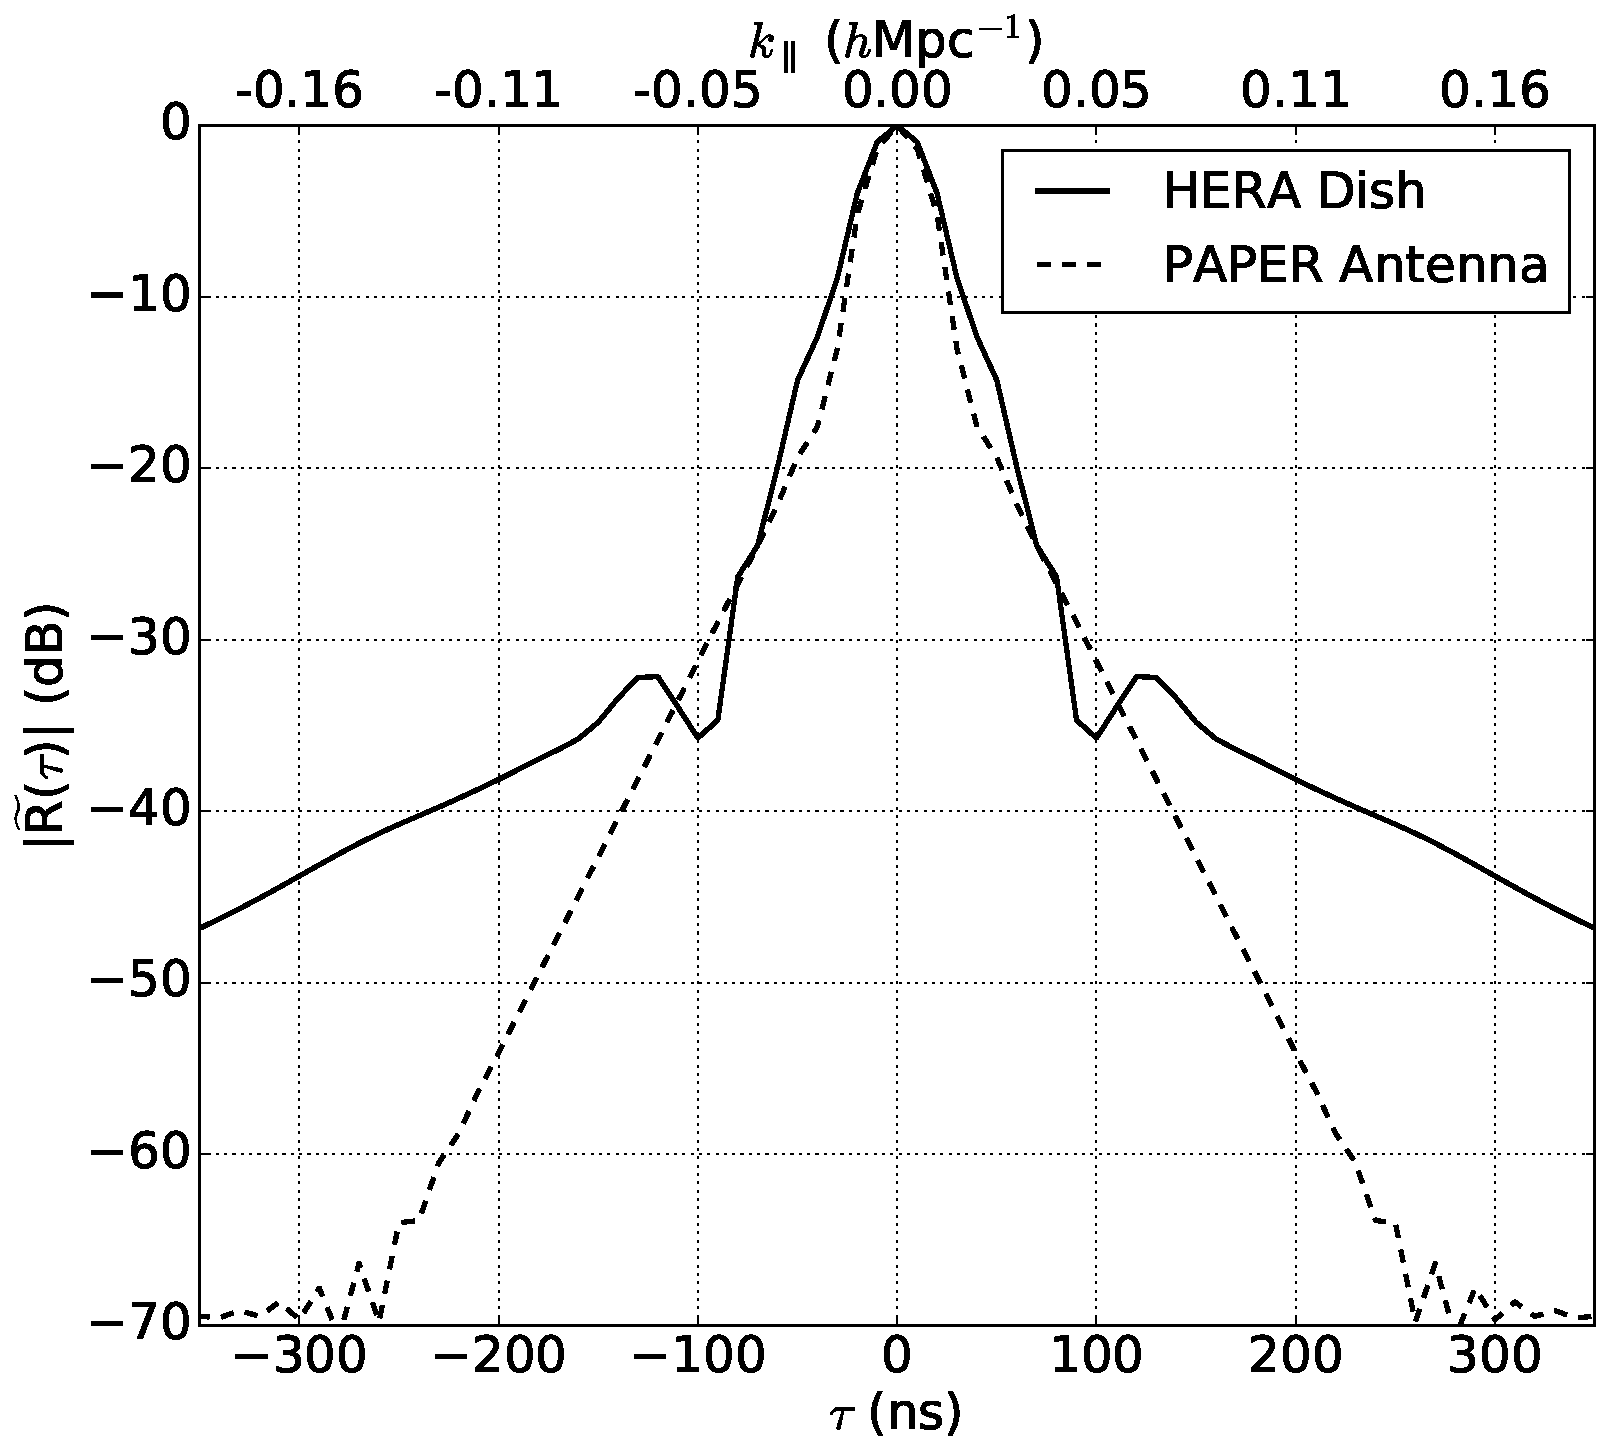
\includegraphics[width=.5\textwidth]{figures/compare_kernels_paper.pdf}
\caption{The response function deconvolved from our simulations (solid lines) compared to the response function estimated from reflectometry measurements described in \citep{Patra:2015} for the HERA dish and the PAPER antenna element. Our simulations agree well with the reflectometry results out to $\approx 100$\,ns but disagree by $\lesssim10$\,dB beyond this. A potential source of the disagreement is uncalibrated structure are irregularities in the cables connecting the Vector Network Analyzer and the antenna feed which enter at the $-50$\,dB to $-30$\,dB level.}
\label{fig:Kernels}
\end{figure}

\subsection{The Delay Response of Subbands}\label{ssec:Subbands}
While we observe a long term falloff due to reflections between the feed and dish element, it is possible that these reflections are localized in frequency and do no effect certain sub-bands. To determine whether the reflections are localized in frequency, we compute the voltage delay response and power kernel for three different subbands: $100-130$\,MHz, $130-160$\,MHz, and $160-190$\,MHz. In order to maintain decent resolution of the kernel itself, we use frequency ranges are larger than the actual subbands that will be used for EoR power spectrum estimation $\sim 10$\,MHz which is set by the interval over which the statistics of the cosmological HI signal are expected to be stationary. We plot the delay transforms of the voltage gain in Fig.~\ref{fig:GainDelaySubbands} and the power kernels in Fig.~\ref{fig:KernelsSubbands}. The central lobe of the delay kernel is significantly wider due to the the wider window functions incurred by the reduced bandwidth, however, the shallow long-term falloff is only visible within the central $125-175$\,MHz band, indicating that long term reflections are isolated near $150$\,MHz and will not effect power spectrum measurements outside of the very center of our band.
To further illustrate the observed isolation of fine frequency structure in the center of the bandpass, we fit the $10$\,MHz intervals of the absolute value of the simulated gains to a sixth order polynomial and compare the residuals in Fig.~\ref{fig:Residuals}. We find that the gain residuals on the sixth order fit are an order of magnitude greater over the $145-155$\,MHz subband than over any other frequency interval. 

\begin{figure}[h!]
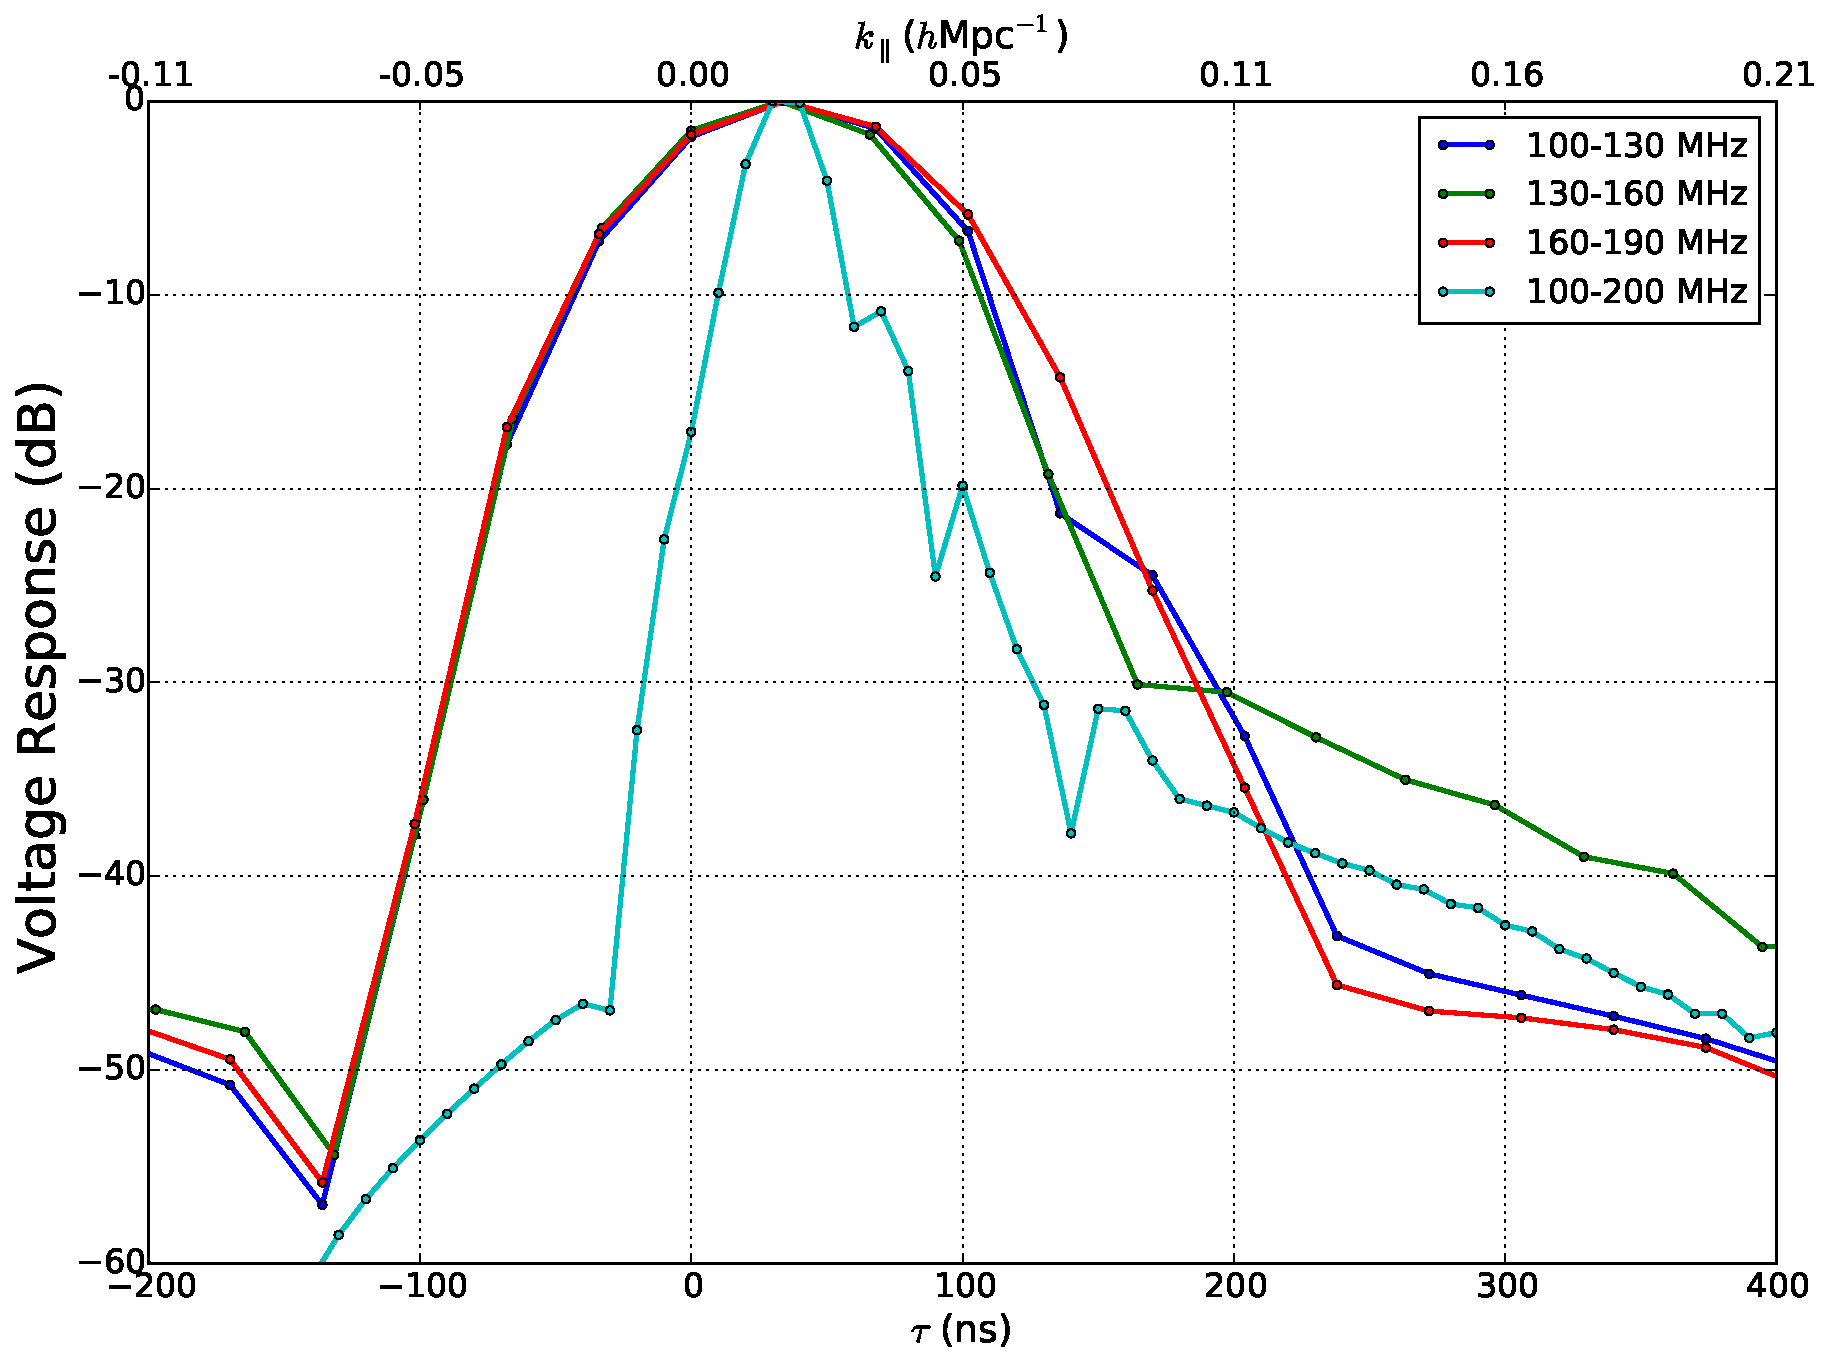
\includegraphics[width=.5\textwidth]{figures/voltageResponseSubbands.pdf}
\caption{The delay transform of the voltage response of the HERA dish for the full 100\,MHz bandwidth (cyan line) along with three subbands; $100-130$\,MHz, $130-160$\,MHz, and $160-190$\,MHz. The shallow falloff observed in \S~\ref{sec:Simulations} is most prominent in the $130-160$\,MHz subband while the falloff in the other subbands is close the the level of the sidelobes (at $\sim -50$\,dB for the lower resolution subbands). $k_\parallel$ values for each delay are computed at $150$\,MHz.}
\label{fig:GainDelaySubbands}
\end{figure}

\begin{figure}[h!]
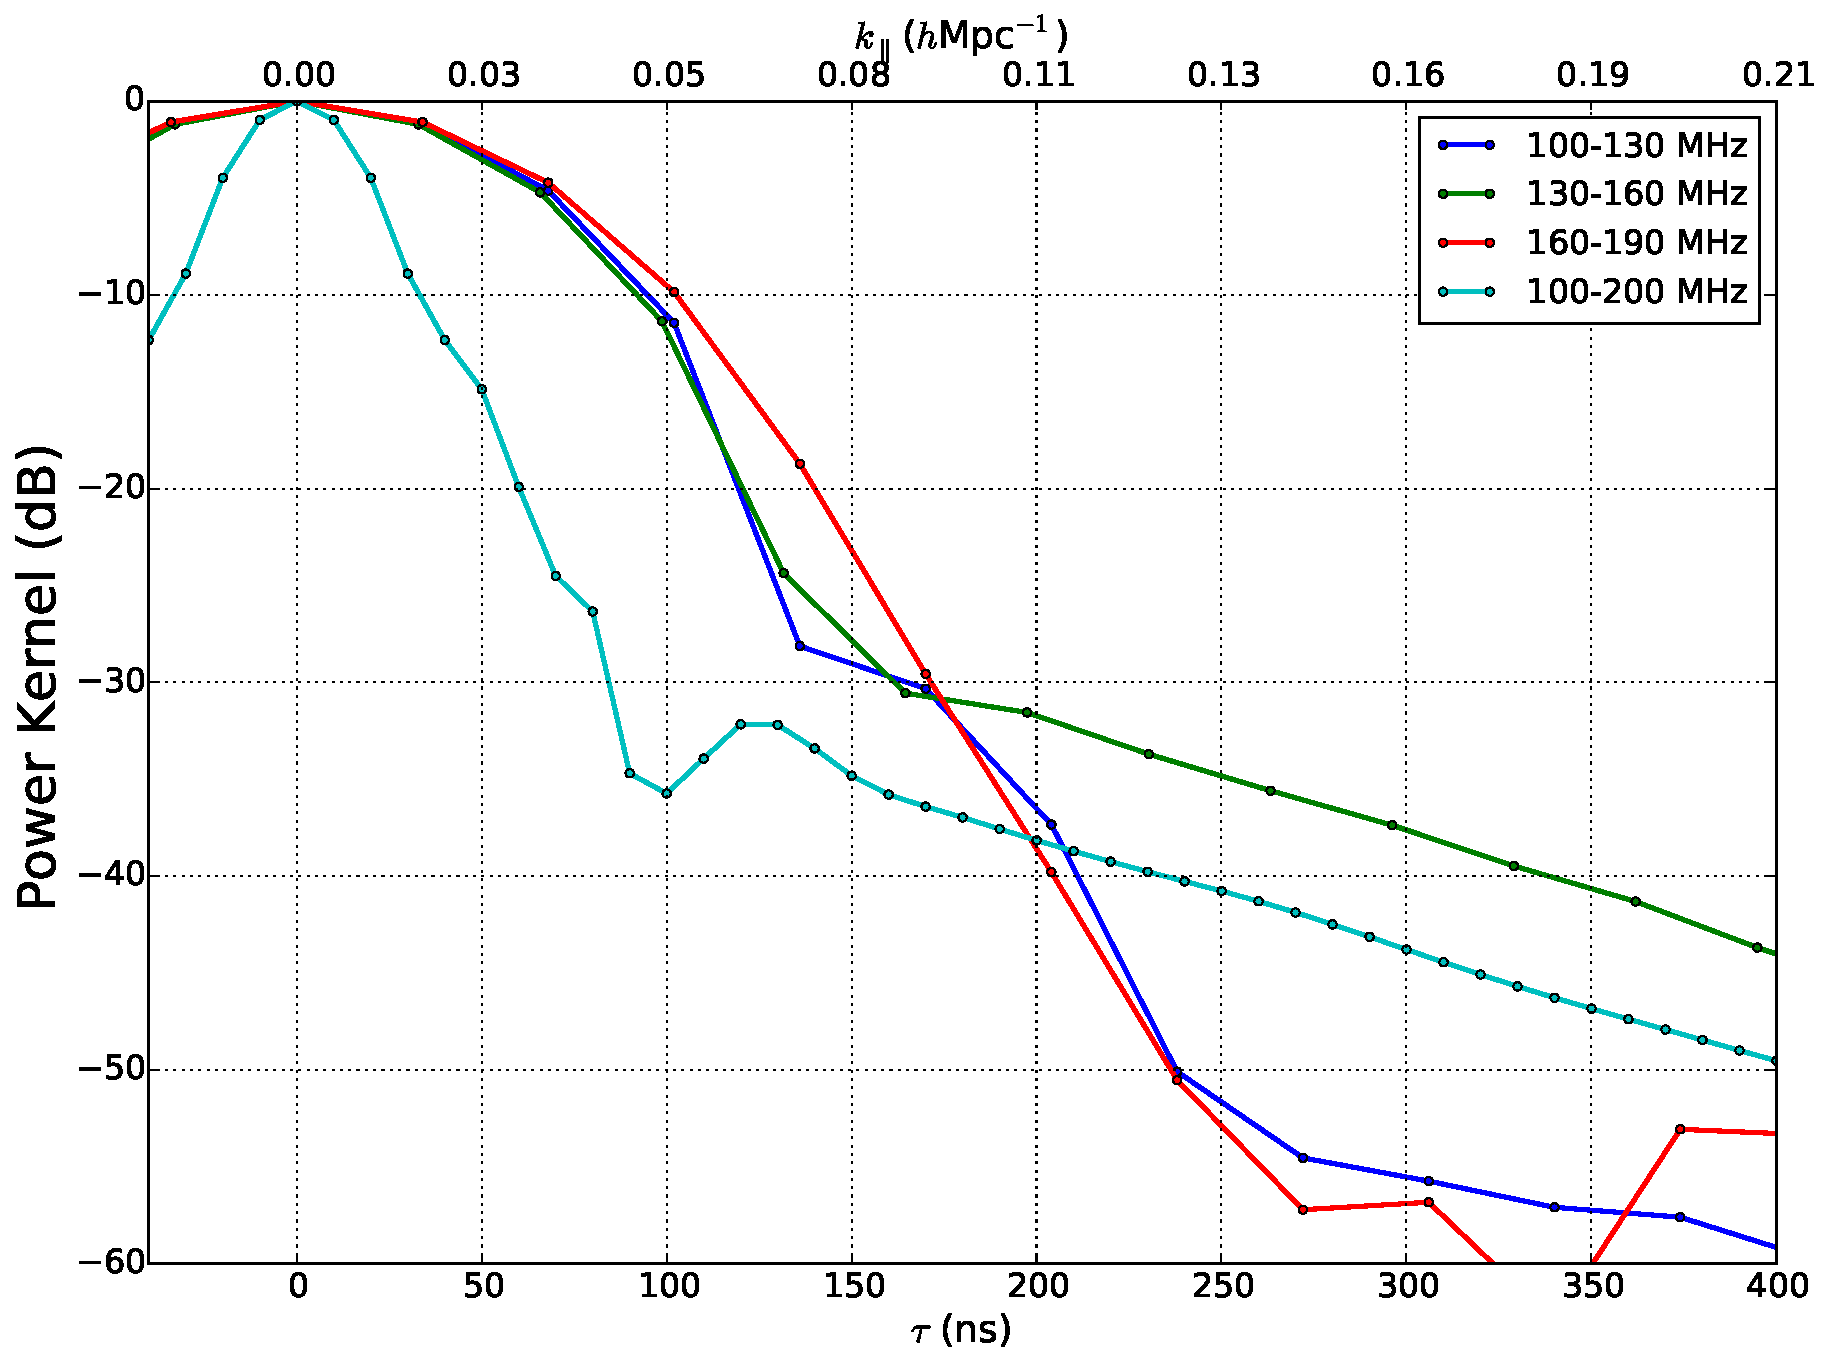
\includegraphics[width=.5\textwidth]{figures/powerKernelSubbands.pdf}
\caption{The power kernel for the three subbands discussed in in \S~\ref{ssec:Subbands} along with the kernel for the full bandwidth response function. While the long term falloff from reflections is prominent between $130-160$\,MHz, it appears at a much lower level in the other two subbands which fall below the central subband by $\sim 20$\,dB at $\sim 300$\,ns. $k_\parallel$ values for each delay are computed at $150$\,MHz. The wider central lobe below 150\,ns for the subband gains is an artifact of the delay resolution of a smaller bandwidth.}
\label{fig:KernelsSubbands}
\end{figure}


\begin{figure*}
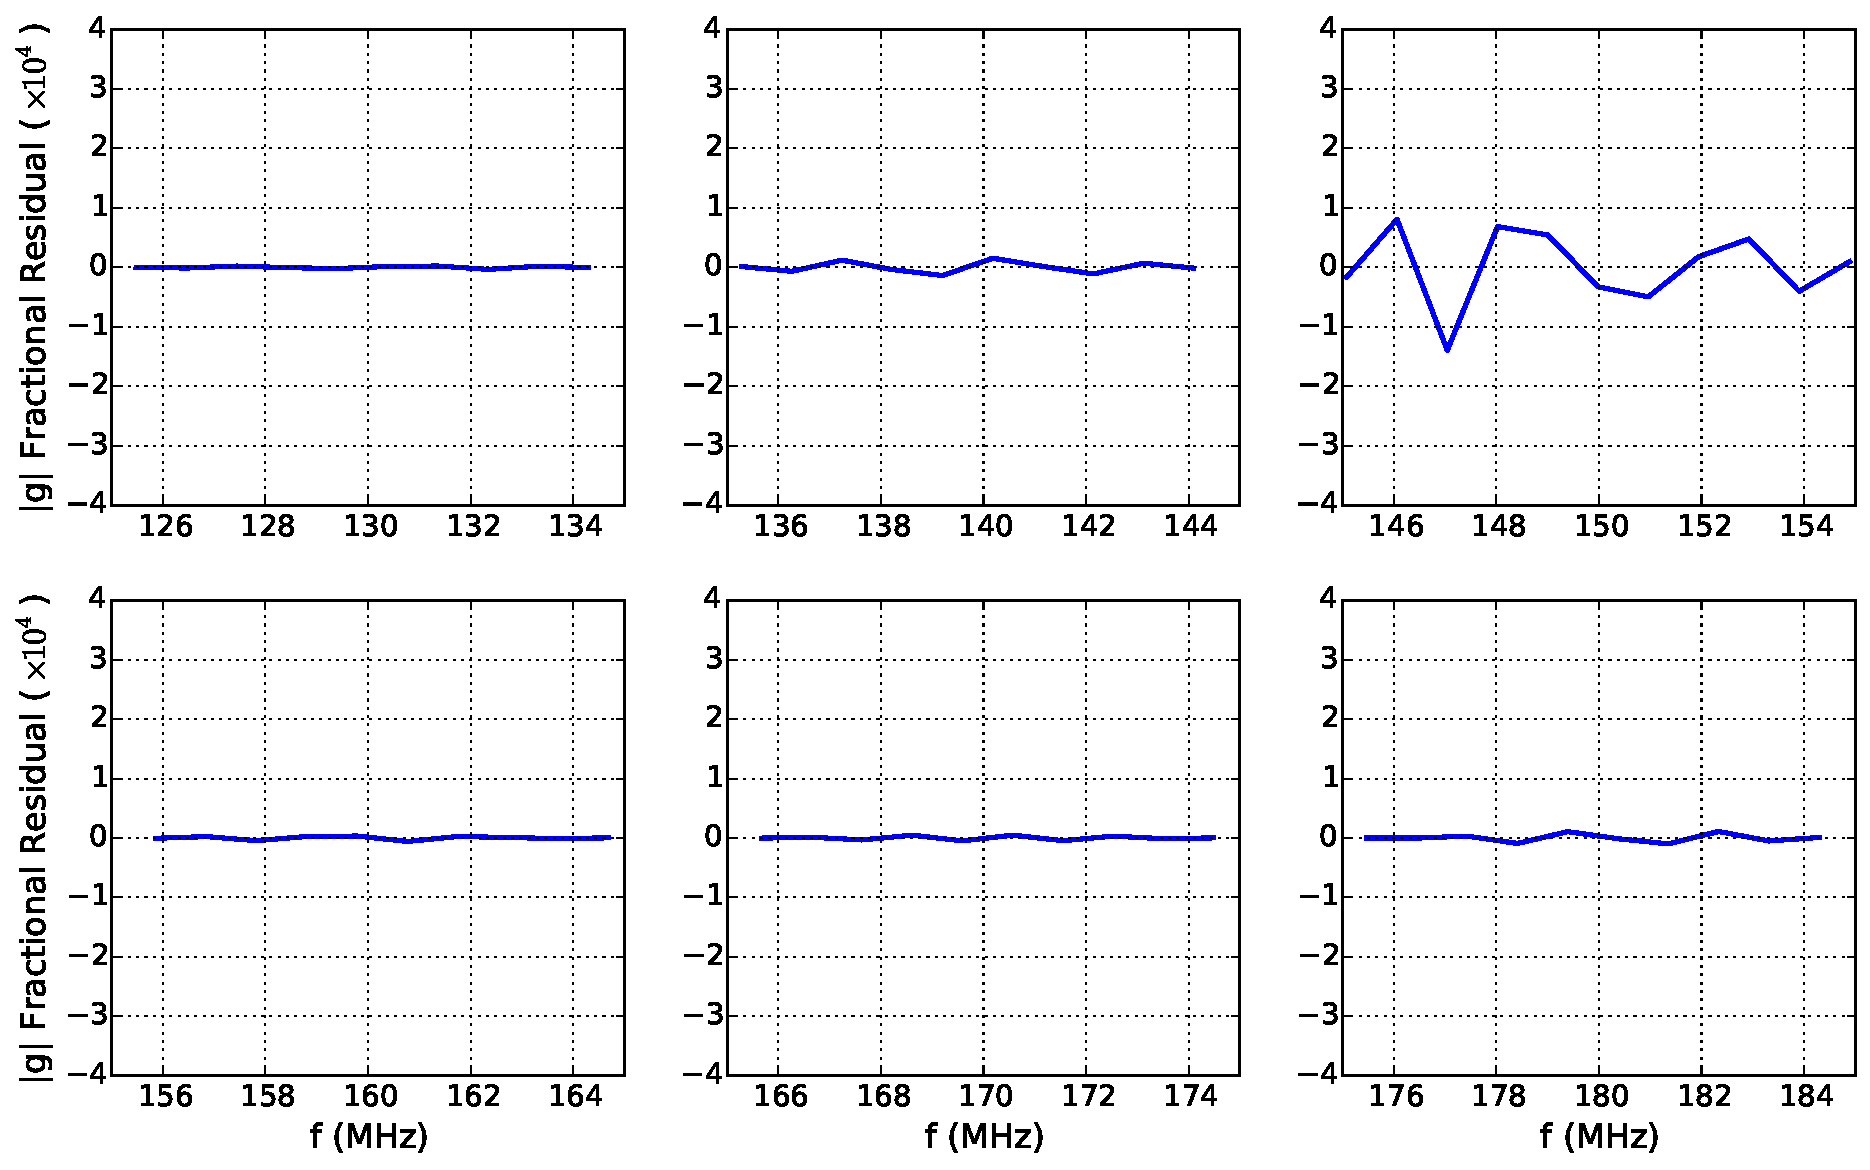
\includegraphics[width=\textwidth]{figures/frequency_domain_residuals.pdf}
\caption{Residuals on the absolute value of the gain over several subbands after fitting to a sixth order polynomial. Consistent with our findings in Fig.~\ref{fig:KernelsSubbands}, the fine frequency residuals in the 145-155\,MHz subband are over an order of magnitude greater than those in the other subbands.}
\label{fig:Residuals}
\end{figure*}


\subsection{Extrapolating the Bandpass and Power Kernel}
Our deconvolution gives us the time-domain voltage response of the PAPER and HERA antenna elements. We plot the absolute value of this response in Fig.~\ref{fig:SimulationsCompare}, seeing that it drops to $-30$\,dB after $\approx 100$\,ns. The power-kernel that convolves visibilities to higher delays is the convolution of $\widetilde{r}(\tau)$ with its time-reversed complex conjugate, which we plot as the red line. The convolution is in very good agreement with the voltage response itself which is explained by the fact that second order terms of the convolution, approximately given by $|\widetilde{r}(\tau)|^2$ (green line) are over two orders of magnitude smaller above $50$\,ns.

Our simulations of the Dish response only extend to $\approx 300$\,ns, however, we wish to understand the impact of reflections on the frequency dependent gain of an interferometer like HERA at comoving scales of $\approx 0.1-0.5$\,$h$Mpc$^{-1}$, corresponding to the delays between 180 and 900\,ns at $z=8$, extending beyond our simulations range. To extrapolate out to higher delays, we assume that the response function is dominated by reflections between the feed and the dish. This is due to the fact that when we extend our filter bandwidth to between $50$ and $250$\,MHz and use a hamming window (which has higher resolution), we observe lobe-like structures at delays beyond $100$\,ns with a periodicity of $30$\,ns, which corresponds to the round-trip light travel time between the feed and the dish.  In addition, the long term falloff appears as a line on a linear-log plot (Fig.~\ref{fig:Simulations}), indicating that the kernel follows an exponential which we now show is indicative of reflections. We do so by adopting the notation of \citep{Patra:2015}. We let $\Gamma_d$ represent the reflection coefficient of the Dish vertex and $\Gamma_f$ represent the reflection coefficient of the feed. An electromagnetic wave incident on the feed, at $t=0$, is accepted with amplitude $(1-\Gamma_f)$. The reflected component travels back to the dish and acquires an amplitude of $(\Gamma_f \Gamma_d)$ before returning at time, $\tau_d$ later where $(1-\Gamma_f)$ will be accepted and so forth. The time dependent voltage at the feed from these reflections is thus
\begin{equation}
\widetilde{v}_r(t) = \sum_m \left( \Gamma_f \Gamma_d \right)^m \widetilde{s}(t-m \tau_d)
\end{equation}
Hence
\begin{equation}
\widetilde{r}_r(\tau) = \sum_m \left( \Gamma_f \Gamma_d \right)^m \delta_D(\tau-m\tau_d)
\end{equation}
Since the number of reflections, $m=t/\tau_d$, than we can write the long-term delay response in discrete form as 
\begin{equation}
\widetilde{r}_n \approx (\Gamma_f \Gamma_d)^{n d\tau/\tau_d}
\end{equation}
which is a power law. We thus model our discrete voltage response beyond the times sampled by our simulations as a power law
\begin{equation}
\widetilde{r} = A X^{(\tau/30\text{ns})} 
\end{equation}
We plot the best power-law fit as a dashed line inf Fig~\ref{fig:SimulationsCompare}.
%We fit our voltage response function and power-kernel to this function, finding a best fit model for the voltage kernel of $A\approx0.95$,$X \approx 0.18$, and $Y\approx 0.58$. The large $Y$ is unrepresentative of the feed reflection coefficient which has been simulated and measured to be $\approx 0.1$ for a head-on EM wave, suggesting that the reflections are arriving from the sides and potentially involve only a small component of the dish and feed. Plotting the die off for the feed reflection coefficient yields dramatically better performance than what is measured.  If the reflections are indeed originating from the sides, and a small component of the dish and feed arrangement, further suppression may be achieved through modifying this component. 


\section{Comparison to Reflectometry Data}\label{sec:Comparison}
\subsection{The Delay Response at Zenith}
In Fig.~\ref{fig:Kernels}, we show the filtered response function deconvolved from our electromagnetic simulations. The response of the dish rapidly dies off as a function of time. After $\approx90$\,ns, we observe lobed structures with a period of $\approx 30$\,ns which corresponds to the geometrical delay between the feed and the dish apex, indicating that the large $\tau$ roll off is dominated by reflections between the feed and the dish. 

Our simulations are intended to verify direct reflectometry measurements taken on a prototype of the HERA feed and dish in Green Bank, presented in \citep{Patra:2015}. For the readers convenience, we briefly explain the reflectometry measurement here before comparing them to our simulation.   

In the reflecometry measurement, a signal is sent from a Vector Network Analyzer (VNA) via a coaxial cable (which is calibrated out) into the back of the feed. The VNA than measures the ratio between returned and transmitted power as a function of frequency, $S_{11}(f)$. A fundamental difference between the reflectometry measurement and the delay response that we are attempting to obtain is that at zero delay, $S_{11}$ is measureing the reflection of the input wave off of the back of the feed while in the delay response of the antenna, the zero delay reflection is the fraction of the electromagnetic wave off of the sky that is accepted by the feed. To obtain $\boldsymbol{\widehat{\rho}}$, we must correct for this difference. It is shown in \citep{Patra:2015} that the correction is 
\begin{equation}
\widehat{\rho}(f) = \frac{\Gamma_a(f)}{1-\Gamma_a(f)} \left[ S_{11}(f) - \Gamma_a(f) \right] + 1 - \Gamma_a(f).
\end{equation}
Applying this transformtion to $S_{11}(f)$ and taking a DFT into the time domain over a band of $100-200$\,MHz, we obtain a measurement based estimate of the dish response function at zenith which is plotted in Fig.~\ref{fig:Kernels} alongside our simulation result. The general trends of the two two lines agree within $\sim 1-3$\,dB. As the long term delay structure of the delay response determines to what extent foregrounds leak out of the wedge, our simulations verify our measurement of the HERA dish's key performance feature.


\subsection{Comparison with the power kernel of the PAPER antenna element}
We next compare the spectral characteristics of the HERA dish to the PAPER antenna element. The PAPER antenna consists of a sleeved dipole element element identical to the one inside of the HERA feed. However, rather than being suspended over a dish which greatly enhances the effective collecting area of the antenna, the dipole is placed facing upwards above a rectangular skirt structure that is designed to minimize spectral structure. Comparing the relative performances of these two configurations is important since by suspending the dipole upside down over a dish, HERA is potentially trading achromaticity for collecting area. Here we comment this tradeoff. In order to perform a comparison, we run an identical plane wave simulation of the PAPER dipole element and obtain the power kernel which is shown in Fig.~\ref{fig:Kernels}. The striking difference between the PAPER and HERA elements is that the PAPER kernel lacks the transition to a shallow falloff at $\sim 100$\,ns which we should expect given that the long term falloff is likely due to feed-dish reflections. {\bf I am here!}
%\begin{figure}
%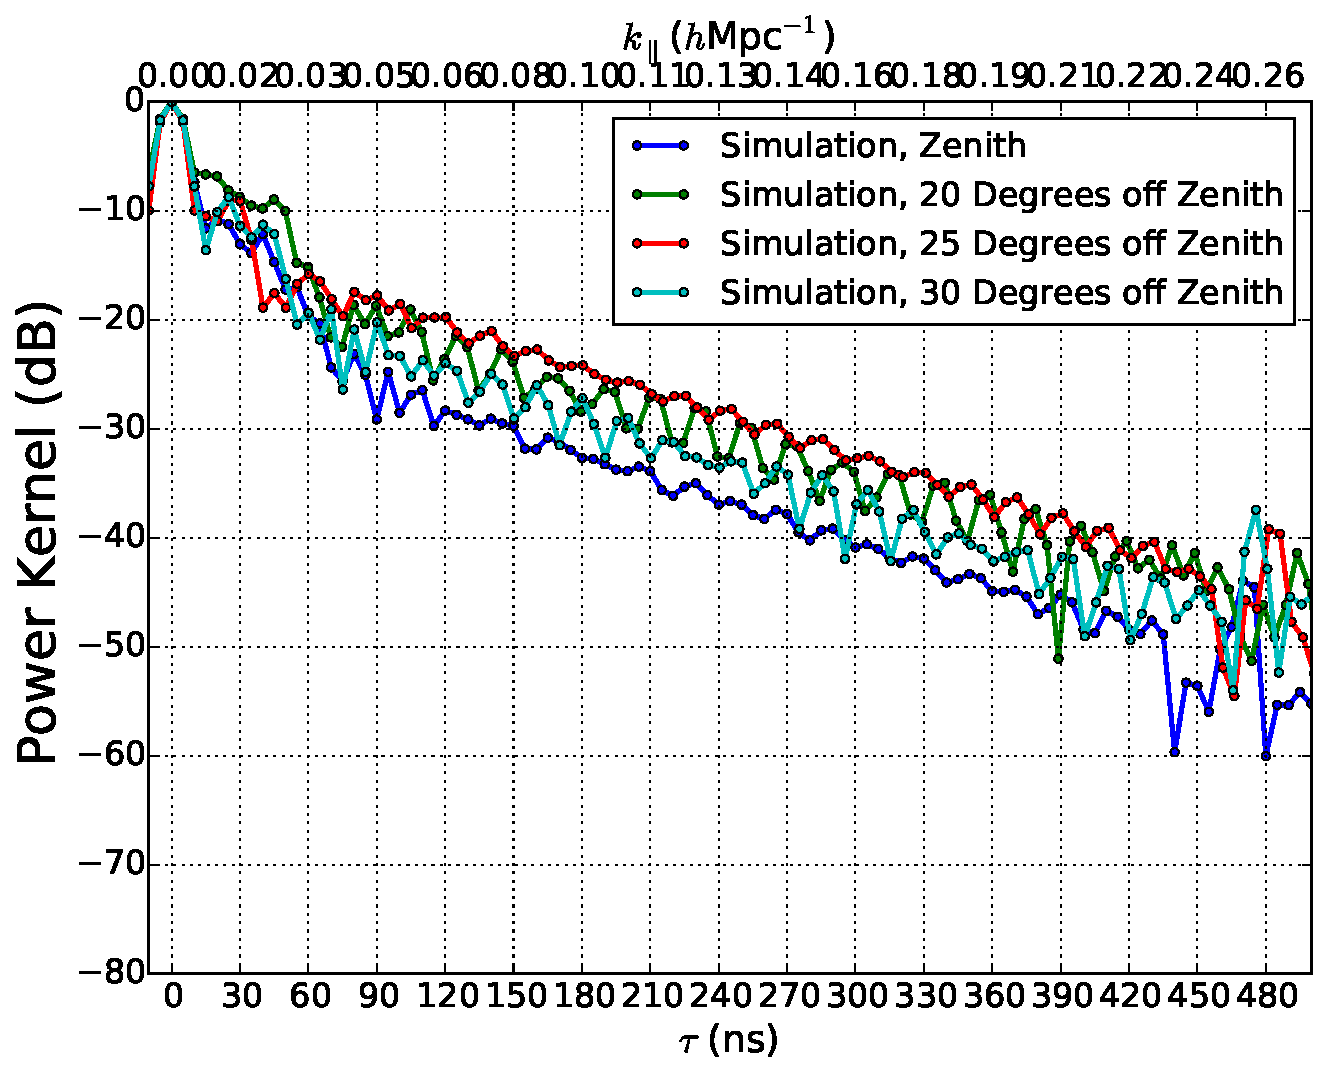
\includegraphics[width=0.5\textwidth]{figures/compareSidelobesNormalized.pdf}
%\caption{The modulus square of the voltage responses of the HERA dish to plane waves incident from zenith (blue line) along with $20^\circ$,$25^\circ$, and $30^\circ$ off-zenith along the NS line. While the sidelobes are suppressed to $\approx 20-25$\,dB at zero delay, they come within $5$\,dB of the zenith response at longer delays which can lead to the level of leakage for a soruce in the sidelobes being comparable to the leakage of a source from zenith. The fact that the sidelobes occupy a much larger solid angle with only moderate supression at $\sim 100$\,ns coupled with their proximity to the horizon, suggests that they will dominate supra-horizon emission.}
%\end{figure}

\section{The Effect of the HERA dish Chromaticity on Foreground Leakage and Sensitivity}\label{sec:Sensitivity}
Having a thorough understanding of how the chromatic beam of the HERA dish leaks foregrounds into higher delays and a decent picture of the relevant voltage response of the dish itself, we are now in a position to explore the impact of the Dish's performance on the leakage of foregrounds beyond the wedge, and into the EoR window. Beyond the delay kernels considered in this paper and \citep{Patra:2015}, the extent of leakage will depend both on the angular structure of the primary beam, which is established in \citep{Neben:2015b} and the model of the foregrounds themselves. In this section, we investigate the amplitude of foreground leakage as a function of delay given an angular primary beam model and our simulation of the delay structure of the dish (\S~\ref{ssec:Leakage}). 

Spectral leakage due to the chromaticity of the dish will cause large-scale LoS Fourier modes to be contaminated by foregrounds and hence inaccessible to the foreground filtering approach that HERA will employ. Since the signal-to-noise ratio is maximized at the smallest $k$ values, the loss of these modes will reduce the significance of the power spectrum detection and negatively impact the overall bottom line of the science that HERA can accomplish. We explore the impact of HERA's intrinsic beam chromaticity on science using the Fisher matrix formalism in \S~\ref{ssec:Science}. 

\subsection{The Impact of the HERA Beam Chromaticity on Foreground Contamination}\label{ssec:Leakage}

Given the HERA dish chromaticity, what Fourier modes will still be accessible with the delay filtering technique? To answer this question, we combine our extrapolated simulations of the HERA dish's spectral structure with simulations of foregrounds. The foreground simulations are described fully in \citep{Thyagarajan:2015c} but for the readers convenience we briefly describe them here. 

Our foreground model consists of two major components: diffuse synchrotron emission from our Galaxy whose structure is described by the Global Sky Model (GSM) of \citet{deOliviaCosta:2008} and a population of point sources sourced by radio loud AGN which combines the NRAO Sky Survey (NVSS) \citep{Condon:1998} at 1.4\,GHz, the Sydney University Mologolo Sky Survey (SUMMS) \citep{Bok:1999} at 843\,MHz, and extrapolate point source fluxes to the observed $100$-$200$\,MHz band using a spectral index of $\langle \alpha \rangle=-0.83$ determined in \citet{Mauch:2003}. Visibilities are computed from the diffuse and point source models assuming the achromatic HERA beam computed at $150$\,MHz and described in \citep{Neben:2015c}. We compute two sets of visibilities: one in which the spectral structure of the dish is assumed to be completely flat, and another in which the beam is multiplied by the Dish's frequency dependent gain at zenith. While this model assumes incorrectly that the frequency evolution of the primary beam is identical along all lines of sight, the majority of power enters at the beams point of maximal gain (zenith) and observations of autocorrelations which reflect the angular average of the frequency dependence of all lines of sight agree well with our simulations at zenith \citep{Patra:2015}. 

The foreground filtering procedure employed by PAPER and HERA involves delay transforming the visibilities on a short time-scale cadence and performing a 1d delay CLEAN where the deconvolution is permitted to discover and subtract foregrounds within the horizon to horizon delay. Since we want to avoid CLEANing noise, the level of foreground subtraction possible by this procedure is limited by the thermal noise level on the visibility, which in terun depends on the number of time steps and redundant baselines that are averaged before performing the cleaning step. In this work, we assume that each visibility is cleaned independently with a two minute CLEANing cadence which corresponds approximately to the time over which HERA's short baselines are coherent. The standard deviation on the real and imaginary part of a single delay transformed visibility is given by \citep{Morales:2004}
\begin{equation}
\Delta V = \frac{\sqrt{2 B} k_B T_{sys}}{A_e \sqrt{\tau}}
\end{equation}
where $A_e$ is the effective area of the dish, $B$ is the bandwidth, $T_{sys}$ is the system temperature, $\tau$ is the integration time, and $k_B$ is the Boltzmann constant. The system temperature can be calculated by assuming that $T_{sys} = 100\text{K} + T_{sky}$ where $100$\,K is the temperature of the PAPER reciever and $T_{sky} = 60 (\lambda/1\,\text{meter} )^{2.55}$ is the sky temperature \citep{Fixsen:2008}. For $A_e$ we use the value of $75$\,m determined in \citep{Neben:2015b}. If we assume that each baseline is cleaned independently and that the integration time is $\tau \approx 60$\,s, than the noise level at 150\,MHz is approximately $9.9$\,Jy\,MHz. In order to avoid subtracting noise, we assume that cleaning is performed down to $5\,\sigma$. In Fig~\ref{fig:Cleaning} we compare the delay transform of visibilities before and after cleaning on a two minute cadence at the LST of 4 hours. While cleaning is able to remove structure within the horizon, it does not reduce any of the power associated with the foreground induced by the chromaticity of the dish. 

To form estimates of the 21\,cm power spectrum, we split each visibility into BlackmanHarris windowed sub-bands centered at redshift intervals of $\Delta z = 0.5$ and each with an equivalent bandwidth of $10\,MHz$, corresponding to the redshift interval over which the statistics of the brightness temperature fluctuations are expected to be stationary. For each windowed interval, we use the flat sky approximation and  Fourier transform in frequency, square, and multiply by a set of prefactors to obtain a power spectrum estimate \citep{Parsons:2014},
\begin{equation}\label{eq:PS}
\widehat{P}({\bf k}) = \left( \frac{2 k_B}{\lambda^2} \right)^2 \frac{X^2 Y}{B_{pp} \Omega_{pp}} | \widetilde{V}({\bf u}) |^2.
\end{equation}
Here, $\lambda$ is the central wavelength of the observation, $k_B$ is the Boltzmann constant, $B$ is the bandwidth of the Fourier transform, and $\Omega_{pp}$ is the integrated solid angle of the primary beam squared. $X$ is a linear factor converting between $uv$ wavelengths and $k_\perp$, and $Y$ is a linear factor converting between $k_\parallel$ and the Fourier dual to frequency, $\eta$. 

A drift scan instrument, HERA will be capable of observing the sky at any LST within the strip declination that passes through its primary beam. To form a final power spectrum estimate, it is expected to perform an average over the power spectrum estimates it obtains through equation~\ref{eq:PS} for each LST independently. It is well documented that foreground power is maximized over certain LST ranges \citep{Thyagarajan:2015a}, hence such an estimate will either filter or weight appropriately the LSTs in which foreground power is maximized. \citet{Thyagarajan:2015c} focuses on the optimal weighting and selection of LST bins in forming a power spectrum estimate. For the purpsoes of our analysis, we focus on a single, relatively clean LST of 4 hours which includes the coldest part of the sky. 




\begin{figure}
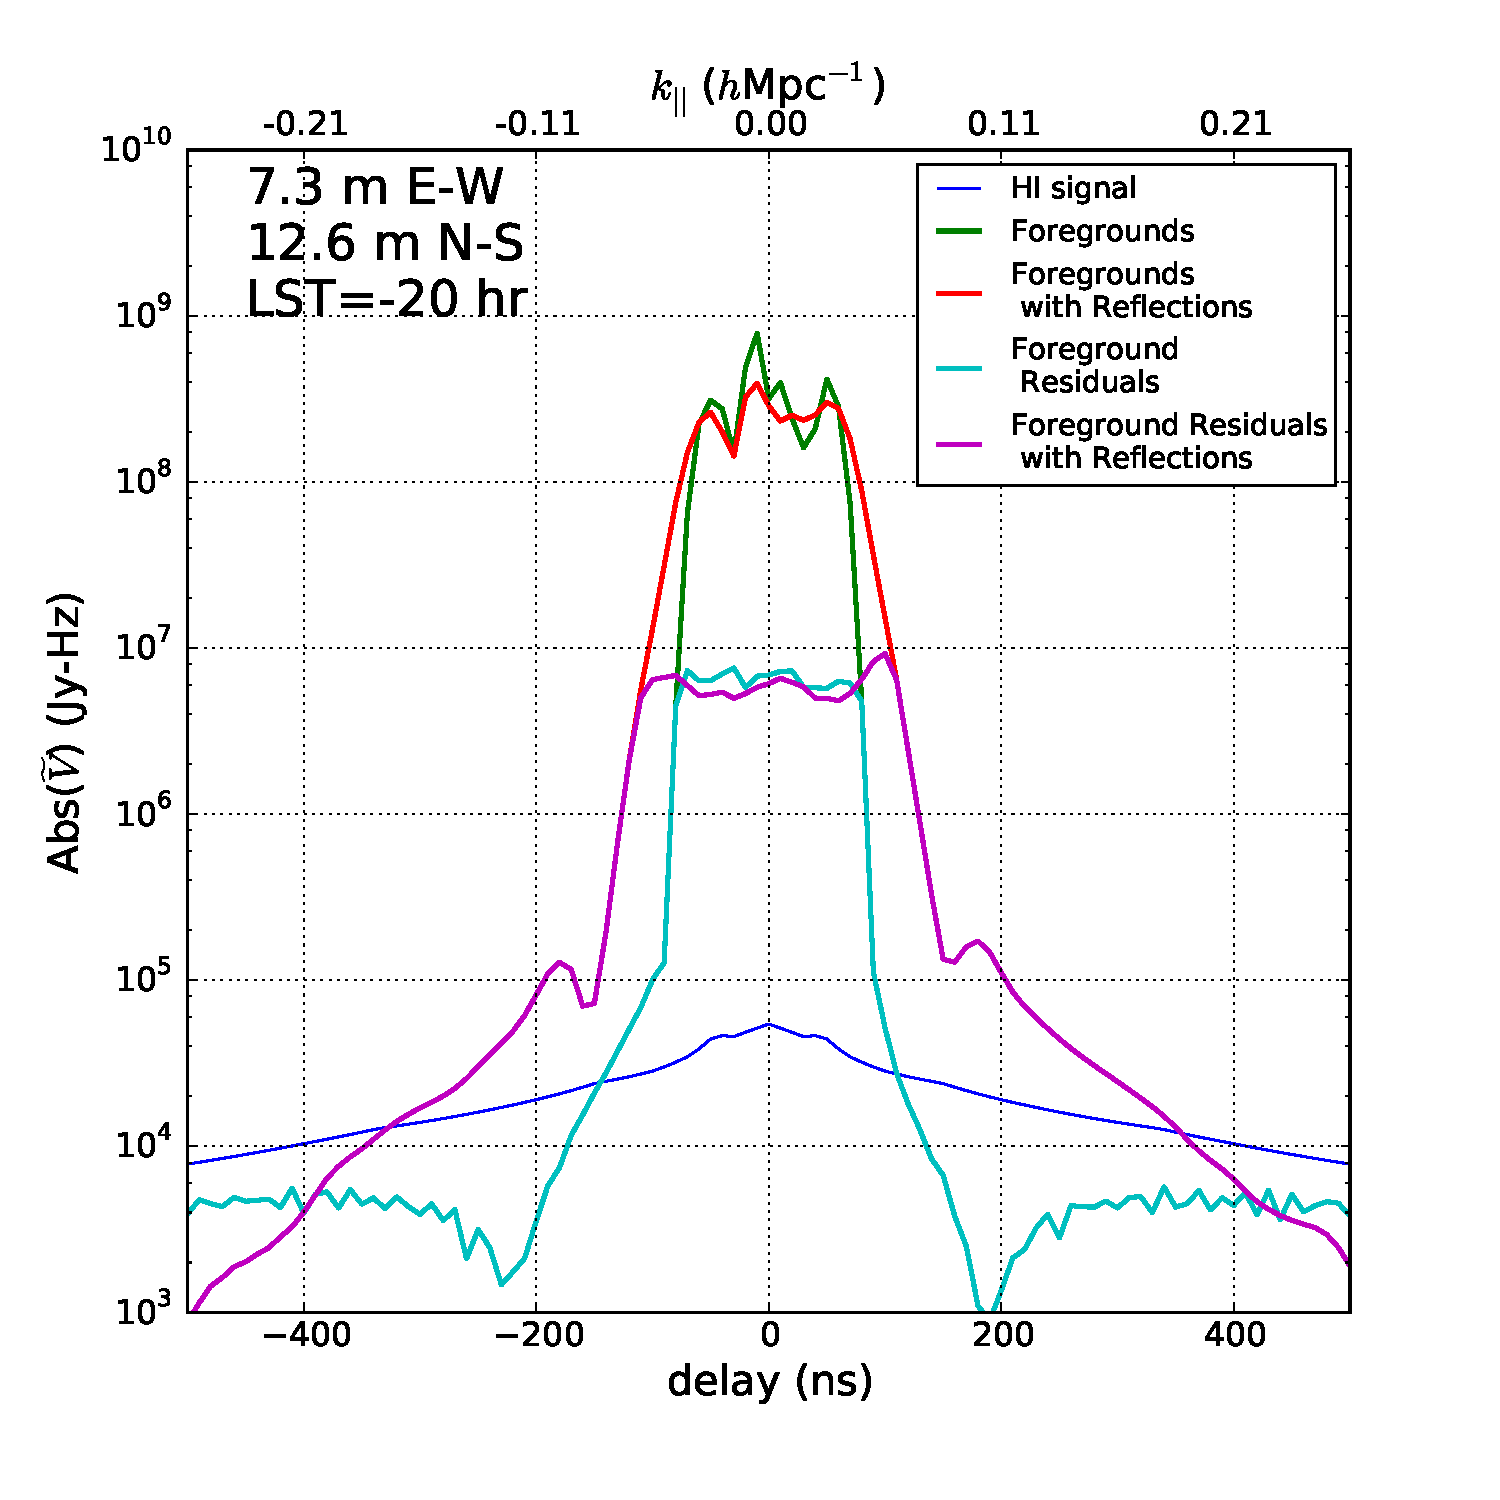
\includegraphics[width=.5\textwidth]{figures/cleaning_noise_Nithya.pdf}
\caption{The absolute magnitude of a delay transformed 14-meter baseline (blue line) compared to the same visibility (green line) contaminated by reflections at the level observed in the HERA dish design. We see that the extended delay kernel smooths out structure, originating from foregrounds, within the horizon. For HERA, we expect to use the delay-clean to remove foregrounds. However, the depth of cleaning is limited by the noise level on a single baseline (black line). We show the foreground residuals with arising from a clean down to the $5\,\sigma$ noise level after 2 minutes of integration, seeing that cleaning at this cadence achieves $\approx$ two orders of magnitude of foreground reduction. The reflections in the dish lead to extensive winged structures that bleed into the EoR window and are well below the thermal noise level. All data in this plot are obtained from a $100$\,MHz bandwidth centered at $150$\,MHz. Vertical dashed lines indicate the horizon delays of the baseline.}
\label{fig:Cleaning}
\end{figure}


Computing the power spectra, we inspect the amplitude of foregrounds given the chromaticity and angular pattern of the HERA dish for several different baselines. We first inspect a $14.6$ and $29.2$ meter baseline in Fig.~\ref{fig:BothBaselines} and find that significant regions of the visibility are foreground free. In both baselines, we find that the residuals after cleaning tend to be at similar levels except at the subband centered at $z=8.5$ (150\,MHz), in which foreground residuals remain above the signal level out to $k_\parallel=0.23$\,$h$Mpc$^{-1}$. Several other baselines especially those oriented entirely in the E-W direction, which we do not show, contain up to two orders of magnitude greater foreground contamination as is noted in \citep{Thyagarajan:2015b}. In a real power spectrum analysis, these baselines would be down-weighted or discarded so that they do not bias our final estimate. 

The level of the foregrounds in Fig.~\ref{fig:BothBaselines} was derived with no attempt to apply inverse covariance weighting \citep{Parsons:2014,Ali:2015} or fringe rate filtering \citep{Parsons:2015}. In order to avoid biases in a maximum likelihood analysis that determines astrophysical and cosmological parameters from our power spectra, the foregrounds should ideally be below the anticipated level of thermal noise which is shown in \citep{Pober:2014} to be on the order of a few percent the anticipated level of the cosmological signal for the full HERA deployment. Hence, as long as we can suppress our foregrounds below 1-10\,\% the signal level, they should not interfere significantly with a maximum likelihood analysis. Thus, the residuals in Fig.~\ref{fig:BothBaselines} serve as a specification for any inverse covariance weighting pipeline which will need to suppress foregrounds by between a factor of $\sim 1-10$ to bring the worst contaminated regions below the level of the signal. Applications of inverse covariance filters in recent PAPER observations have yielded improvements at and above this level, hence our simulations show that even with the presence of beam chromaticity, HERA will be able to isolate foregrounds below below the level of thermal noise in most of the EoR window. 

\begin{figure*}
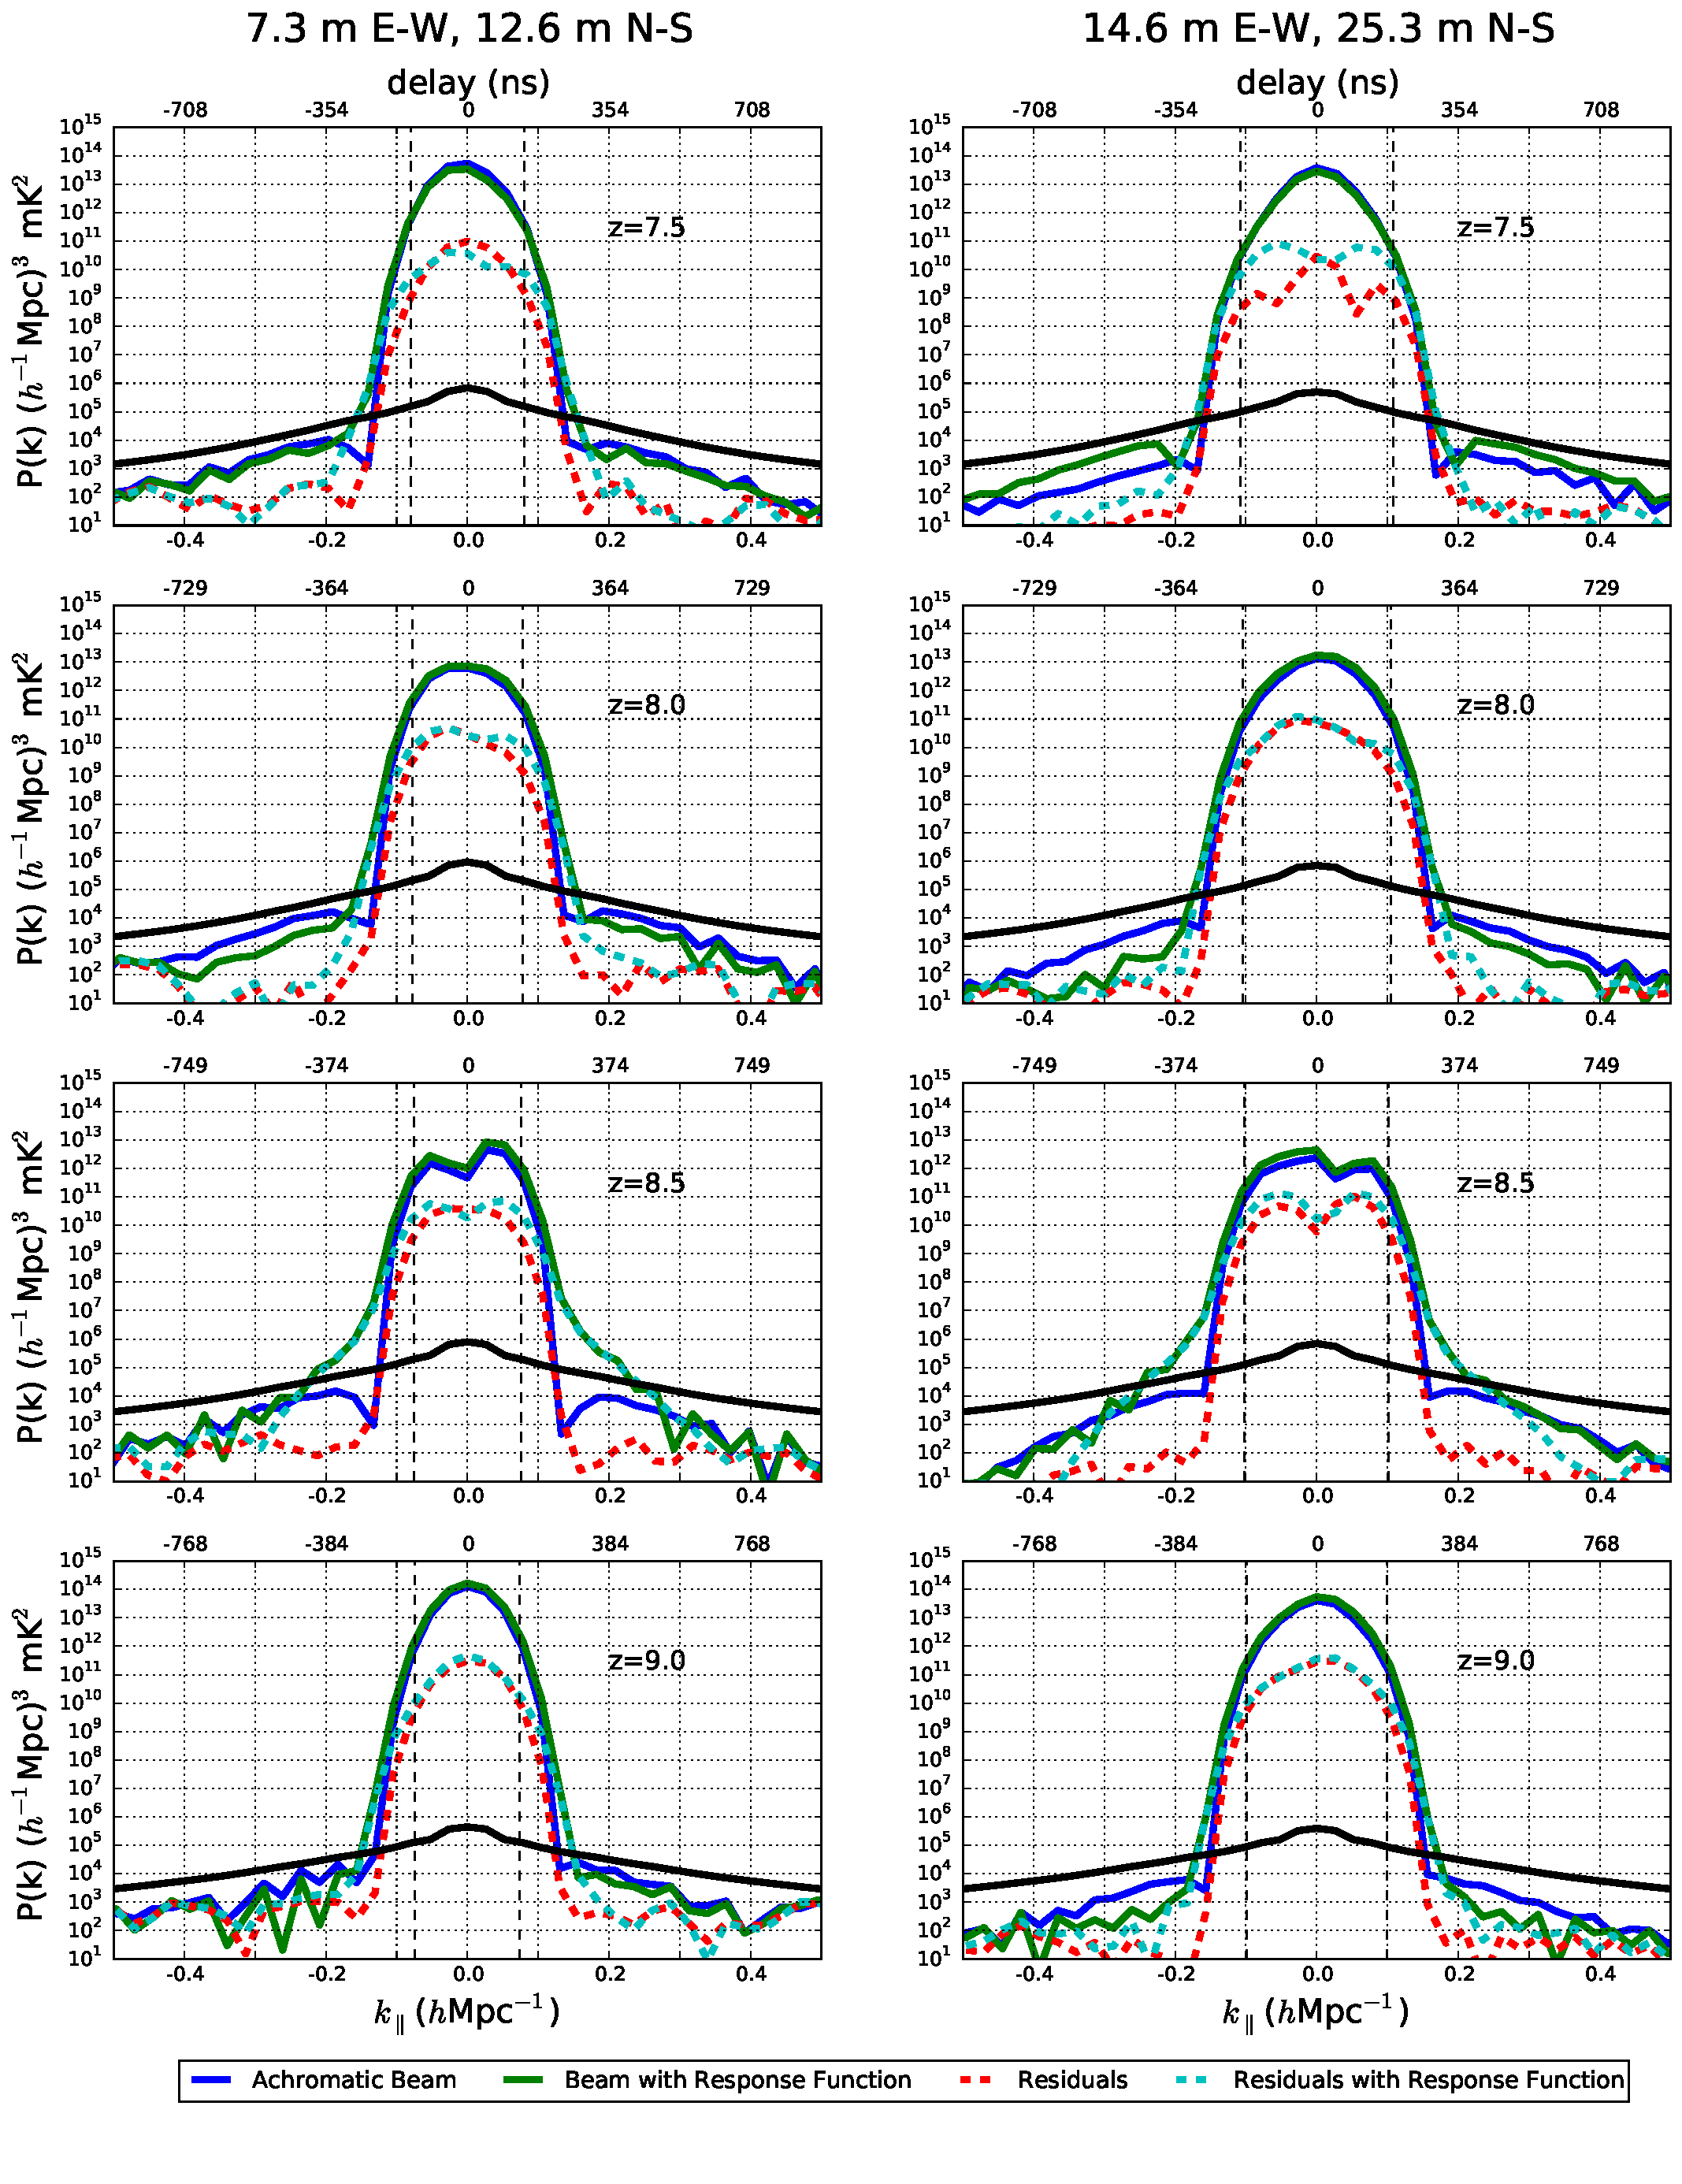
\includegraphics[width=\textwidth]{figures/ps_compare_nithya_bothBaselines.pdf}
\caption{}
\label{fig:BothBaselines}
\end{figure*}


%\begin{figure*}
%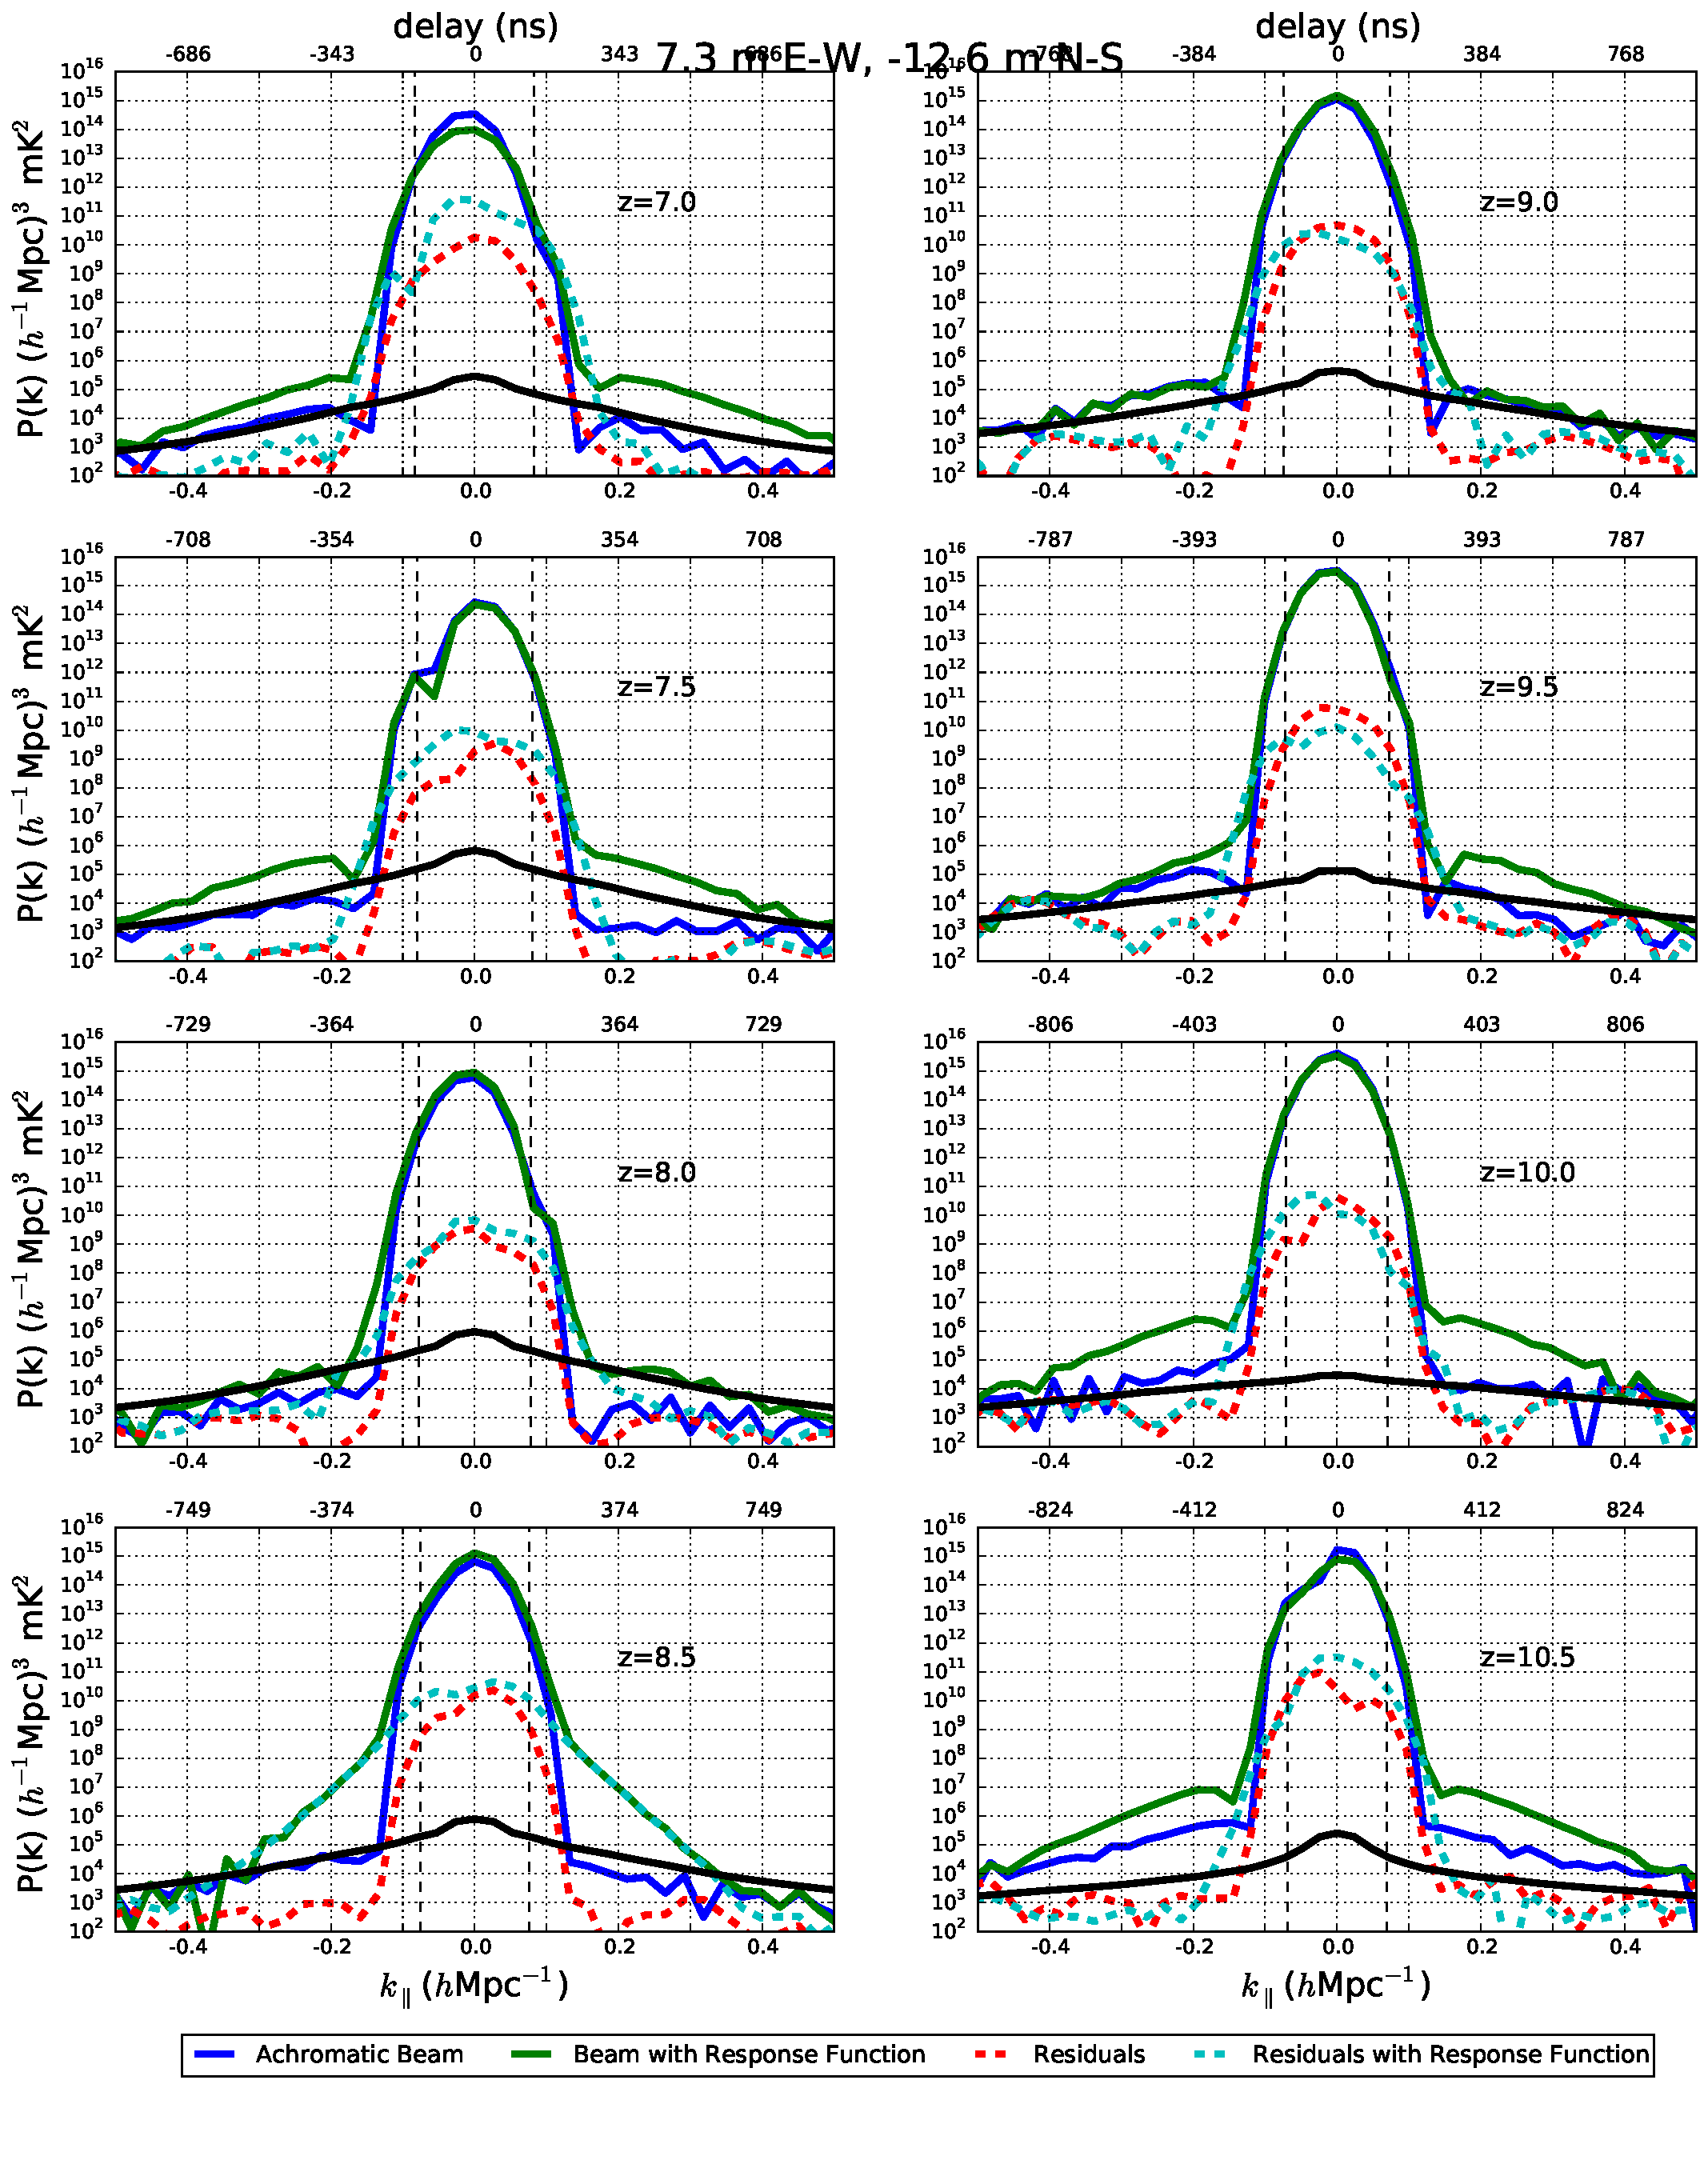
\includegraphics[width=\textwidth]{figures/ps_compare_nithya_lst4hr_1024ch_7p3ew_12p6ns.pdf}
%\caption{The power spectrum computed from the delay transform of a 14.6 meter baseline in equation~\ref{eq:PS} with (solid green line) and without (solid blue line) the presence of reflections in the HERA dish. The residuals after cleaning within the dashed black lines down to three times the level of thermal noise after 20 minutes of integration with (dashed cyan) and without (red dashed) the dish chromaticity are also plotted. We find that for this short baseline, clean residuals are on a similar level as the 21\,cm signal (solid black line), indicating that a redesign of the array with fewer short baselines may be necessary to maximize its sensitivity on foreground free modes.}
%\label{fig:shortBaseline}
%\end{figure*}


%\begin{figure*}
%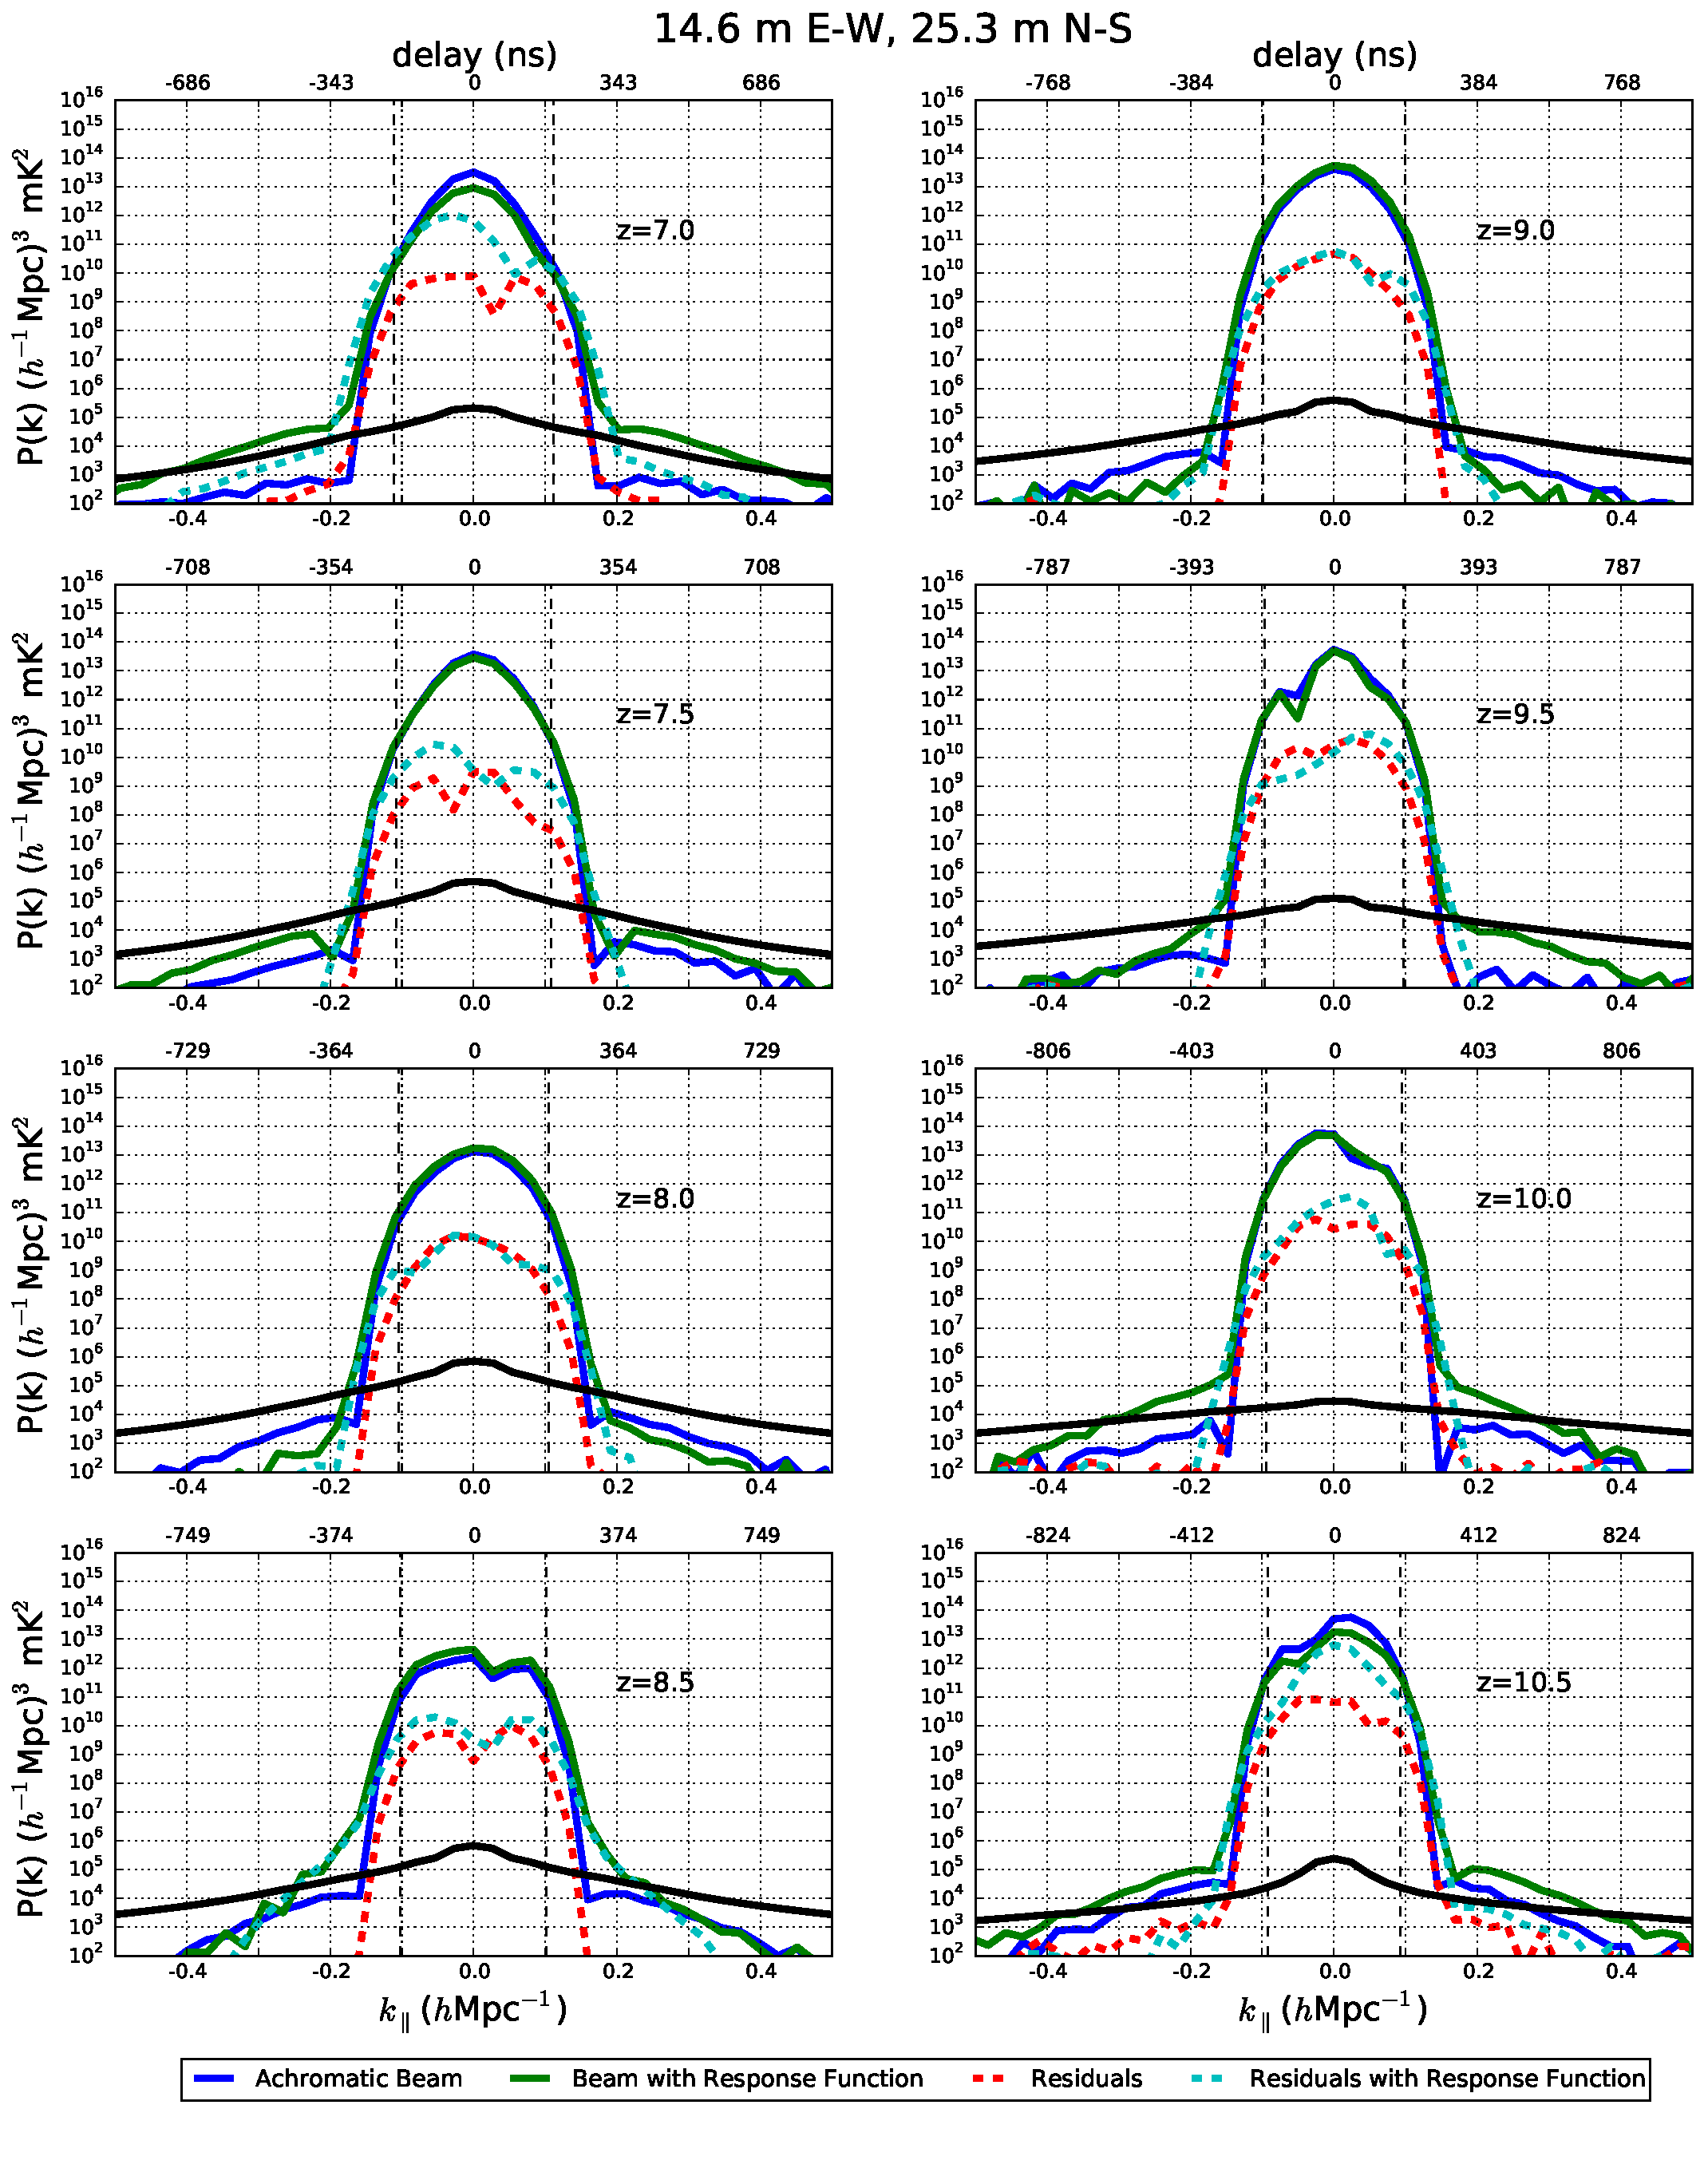
\includegraphics[width=\textwidth]{figures/ps_compare_nithya_lst4hr_1024ch_14p6ew_25p3ns.pdf}
%\caption{The same as Fig.~\ref{fig:shortBaseline} except now for a 29.2 meter baseline. We see that the level of foregrounds is down relative to our 14.6 meter baseline by two orders of magnitude, likely due to the fact that we are now outside of the region with significant contamination from the Galaxy. The presence of reflections tends to extend the $k_\parallel$ at which foregrounds drop below the level of the signal between $k_\parallel=0.15$\,$h$Mpc$^{-1}$ and $k_\parallel=0.22$\,$h$Mpc$^{-1}$ with the most severe contamination occurring at the $z=8.5$ subband where the reflections where observed to be worst in Fig.~\ref{fig:KernelsSubbands}. }
%\label{figure:shortBaseline}
%\end{figure*}

%\begin{figure*}
%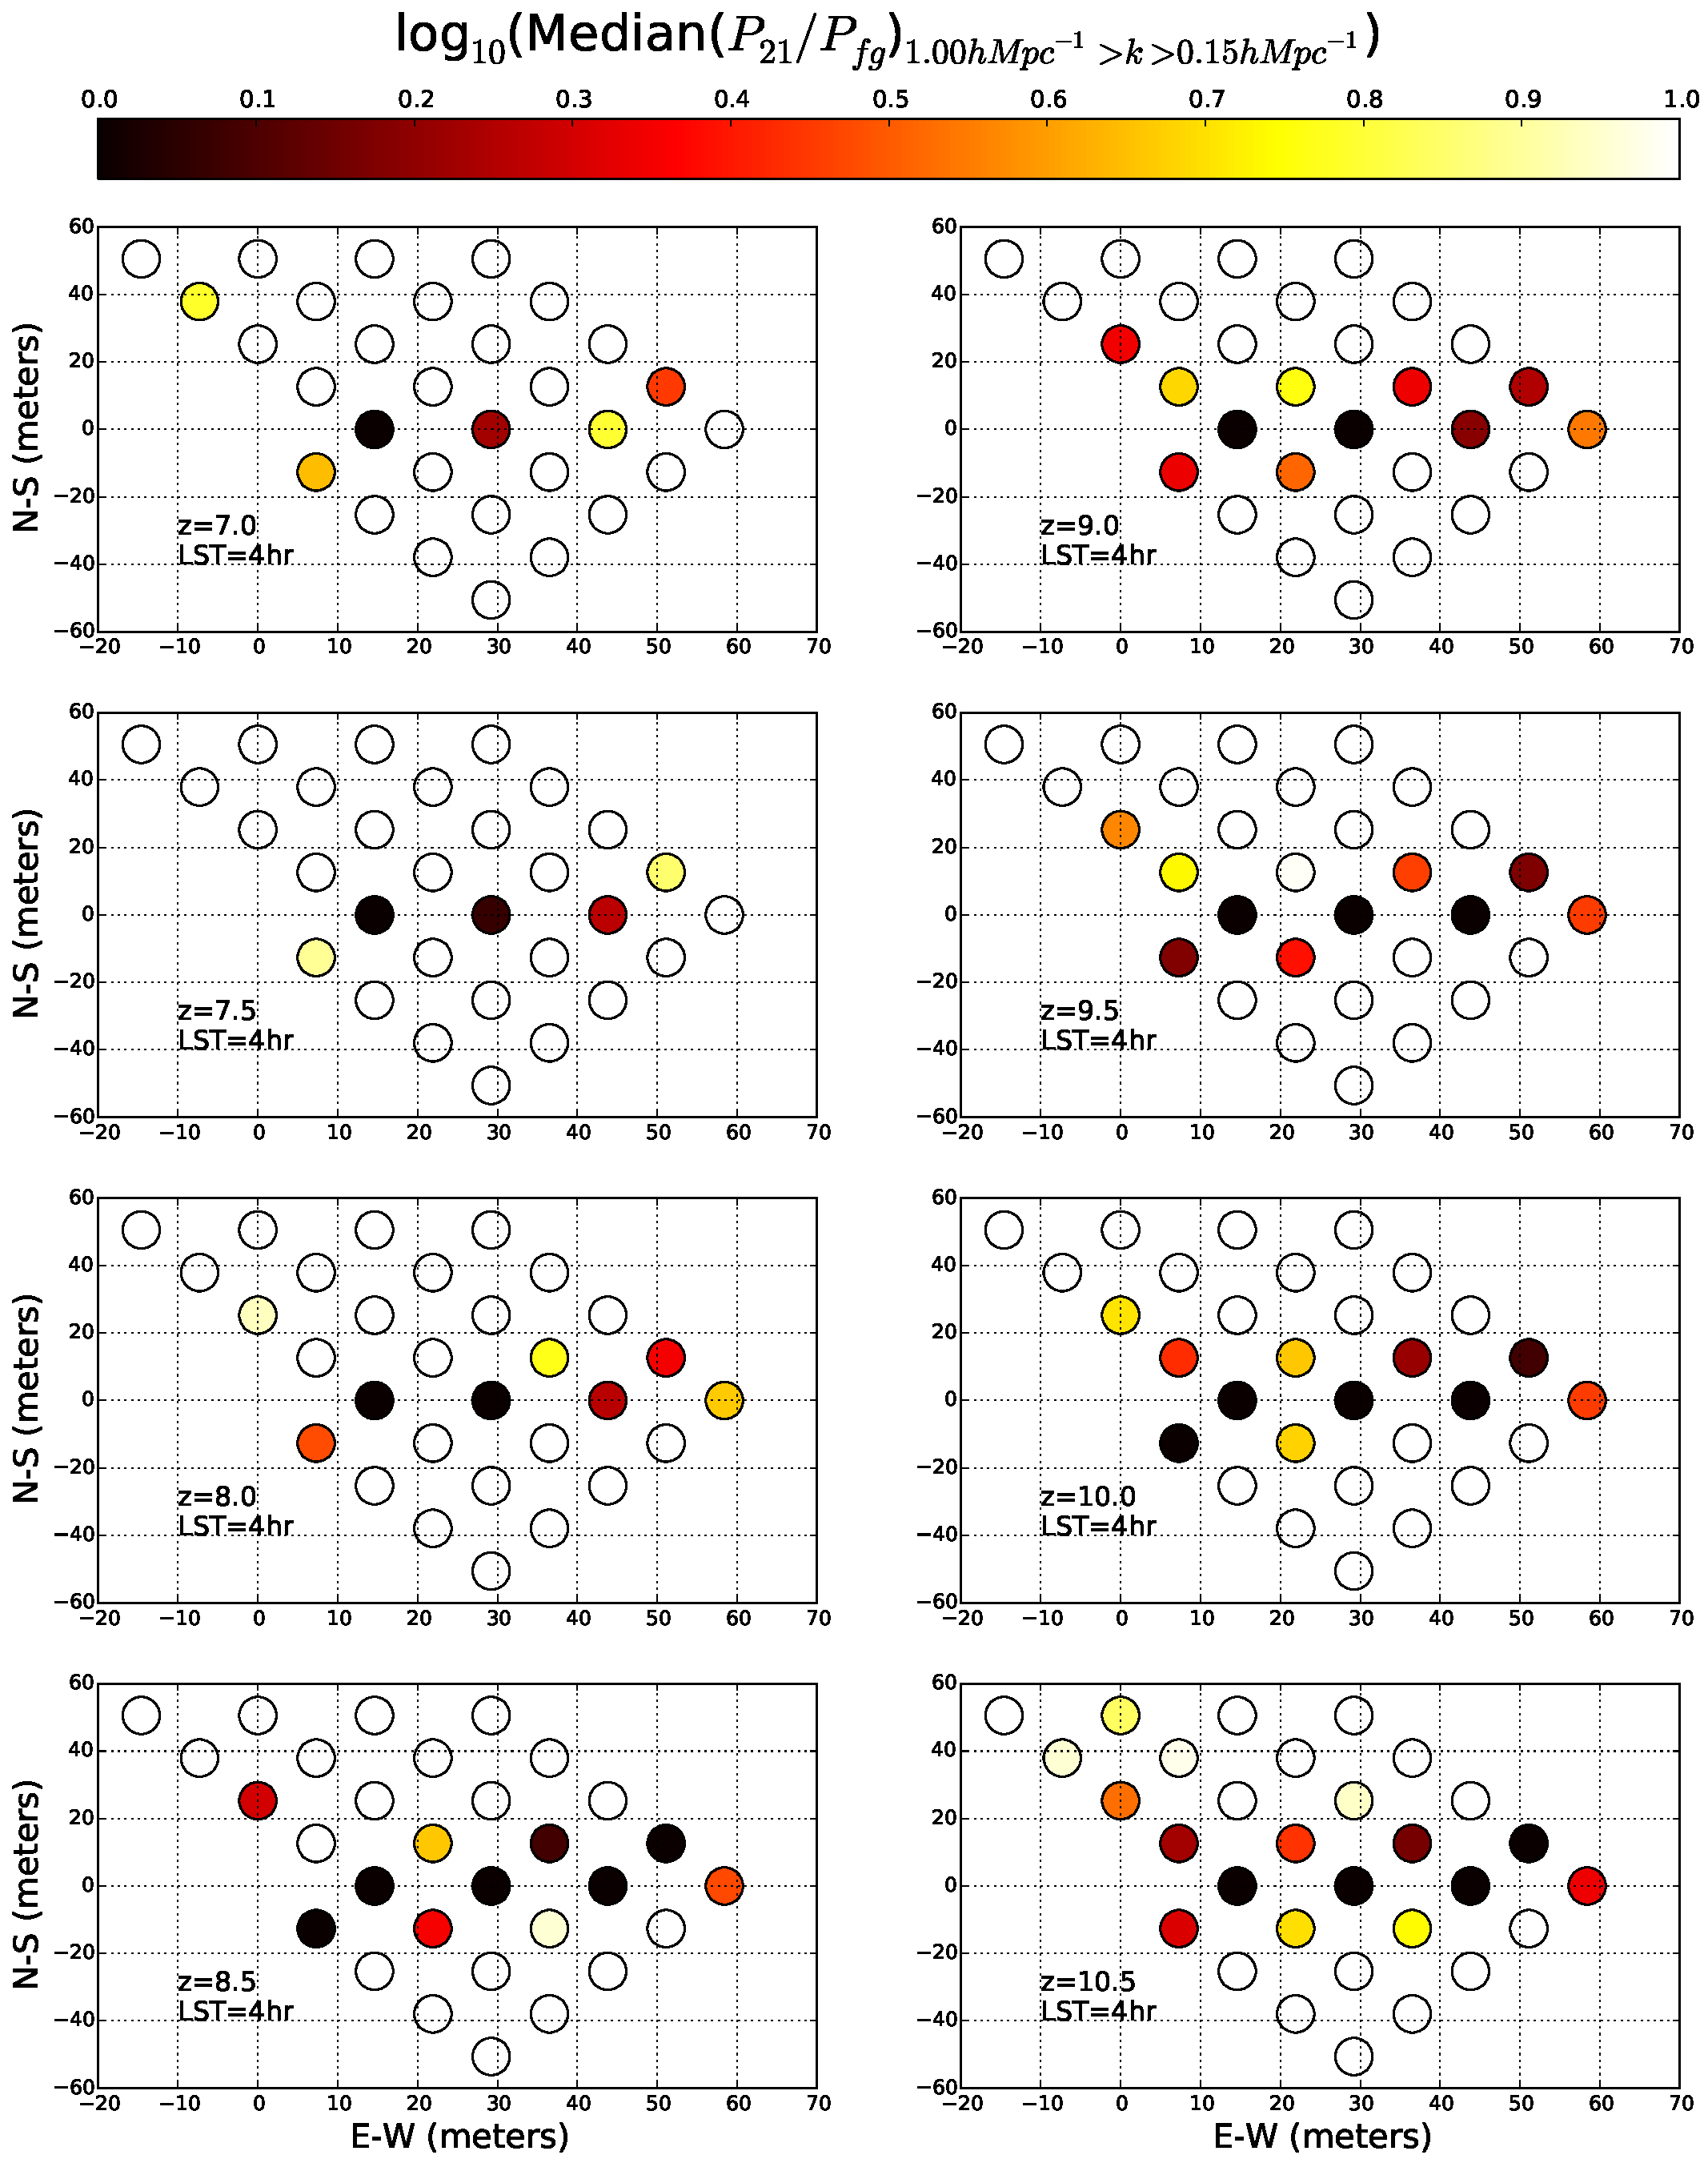
\includegraphics[width=\textwidth]{figures/ps_compare_nithya_lst4hr_snrVbaselineMedian.pdf}
%\caption{The median of the ratio between foreground residuals with the chromaticity of the HERA primary beam between $k_\parallel=0.15$\,$h$Mpc$^{-1}$ and $k_\parallel=1.0$\,$h$Mpc$^{-1}$, the range of k values over which HERA will derive the majority of its sensitivity. We see that the shortest baselines tend to have relatively low signal to foreground ratios due to the presence of high amplitude Galactic synchrotron emission.}
%\label{fig:Medians}
%\end{figure*}

\subsection{The Implications of Dish Reflections on EoR Science}
The primary goal 21\,cm EoR observations is to obtain information about the nature of the sources that drove reionization. Since the amplitude of the 21\,cm signal is maximal at smaller $k$ values, a loss of large scale signal due to foreground leakage eliminates the the modes that HERA would otherwise have the greatest signal to noise detections, impacting our overall sensitivity and its ability to derive this information. In this section, we estimate the impact of foreground leakage on HERA's sensitivity along with its ability to determine the astrophysics of reionization. We do so using the Fisher Matrix formalism. The Fisher Matrix allows us to forecast the covariances and errors on reionization parameters given errors on power spectrum observations due to the uncertainties caused by thermal noise which is in turn determined by the $uv$ coverage and observing time of the interferometer. The covariance between the parameters of some model ${\bf \theta}$ is given by the inverse of the Fisher matrix, ${\bf F}$ which for Gaussian and independently determined power spectrum bins may be written approximately as \citep{Pober:2014,EwallWice:2015a},
\begin{equation}\label{eq:Fisher}
F_{ij} \approx \sum_{k,z} \frac{1}{\sigma^2(k,z)} \frac{\partial \Delta^2(k,z)}{\partial \theta_i} \frac{\partial \Delta^2(k,z)}{\partial \theta_j},
\end{equation}
where $\Delta^2(k,z)$ is the power spectrum amplitude for some $k-z$ bin and $\sigma^2(k,z)$ is the variance of the power spectrum estimate in that bin due to thermal noise and cosmic variance \citep{Beardsley:2013}. 

 we use the publicly available {\tt 21cmFAST} code \citep{Mesinger:2011} which generates realizations of the 21\,cm brightness temperature field using the excursion set formalism of \citet{Furlanetto:2004}. We employ a popular three parameter model of reionization \citep{Mesinger:2012,Pober:2014,Greig:2015,Liu:2015} with the following variables 
\begin{itemize}
\item ${\bf \zeta}$: The ``ionization efficiency" is defined in the \citep{Furlanetto:2004} excursion formalism to be the inverse of the mass collapse fraction necessary to ionize a region and is computed from a number of other physical parameters such as the fraction of collapsed baryons that form stars and the UV photon escape fraction. Because $\zeta$ acts as an efficiency parameter, its primary affect is to change the timing of reionization. We choose a fiducial value of $\zeta=20$, though its possible values range anywhere between $5$ and $50$. 
\item ${\bf R_\text{mfp}}$: The presence of Lyman limit systems and other potential absorbers within HII regions causes UV photons to have a mean free path denoted by $R_\text{mfp}$. In the {\tt 21cmFAST} framework, HII regions cease to grow after reaching the radius of $R_\text{mfp}$, primarily impacting the morphology of the signal. We choose a fiducial value of $R_\text{mfp}=15$\,Mpc which is in line with recent simulations accounting for the subgrid physics of absorption \citep{Sobacchi:2014}. 
\item ${\bf T_\text{vir}^\text{min}}$: The minimal mass of dark matter halos that hosted ionizing sources. While in principle, halos with virial temperatures as small as $10^2$\,K are though, in principle, to be able to form stars, thermal and mechanical feedback have been seen to raise this limit to as high as $10^5$\,K. We choose a fiducial value of $T_\text{vir}^\text{min} = 1.5\times 10^4$\,K which is set by the atomic line cooling thresshold. 
\end{itemize}
In order to account for the degeneracies in the power spectrum between heating from X-rays and reionization from UV photons, we also marginalize over three additional parameters that describe the impact of heating from early X-ray luminous sources as explored in \citep{EwallWice:2015b}. These are the X-ray heating efficiency $f_X$, the maximal energy of X-ray photons that are self absorbed by the ISM of early galaxies, $\nu_\text{min}$, and the spectral slope, $\alpha$ which are taken to have fiducial values of $1$,$0.3$\,keV, and $-1.2$ respectively. We choose to parameterize our model in terms of the fractional differences of each parameter from their fiducial values so that, for example, $\theta_\zeta = (\zeta - \zeta_\text{fid})/\zeta_\text{fid}$ and compute the derivatives in equation~\label{eq:Fisher} by performing a linear fit to realizations of the 21\,cm power spectrum calculated by {\tt 21cmFAST} at $\theta_i= \pm 10^{-2}, \pm 5\times 10^{-2}, \pm 10^{-1}$,and $ \pm 2 \times 10^{-2}$. 

What about $\sigma^2(k,z)$? $\sigma^2$ represents the noise on each 1 dimensional power spectrum estimate. For each measurement in the $uv$ plane, the standard deviation of a power spectrum measurement is given by the direct sum of sample variance and thermal noise \citep{McQuinn:2006} which in turn depends on the primary beam of the instrument and the time spent sampling each $uv$ cell. For our analysis, we assume that the $uv$ plane is sampled by circular apertures with effective areas of $75$\,m$^2$ and that $\tau({\bf k})$ is determined by by a drift scan in which baselines are integrating coherently on each $uv$ cell for $\approx 20$\,minutes. 


\begin{figure}
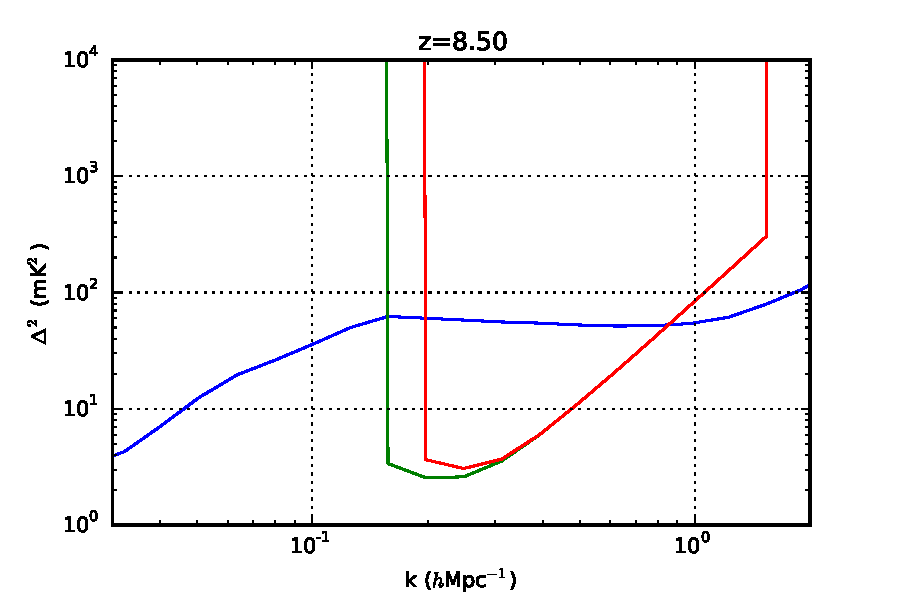
\includegraphics[width=.5\textwidth]{figures/sensitivity_comparison_v2.pdf}
\caption{A comparison between the sensitivity achieved by HERA at redshift $8.5$ with and without the presence of beam chromaticity due to the reflections studied in this work. We saw in Fig.~\ref{fig:BothBaselines} that with reflections, foregrounds exceed the signal level out to $k=0.2$\,$h$Mpc$^{-1}$ at $z=8.5$ which we assume are unusable, forcing us to ignore modes out to $350$\,ns beyond the horizon, leading to the sensitivity projected in the red curve. The absence of these reflections allows us to work within $250$\,ns of the horizon (green curve), leading to an increase in sensitivity by a factor of $\approx 1.5$. }
\label{fig:Sensitivity}
\end{figure}



\begin{figure*}[h!]
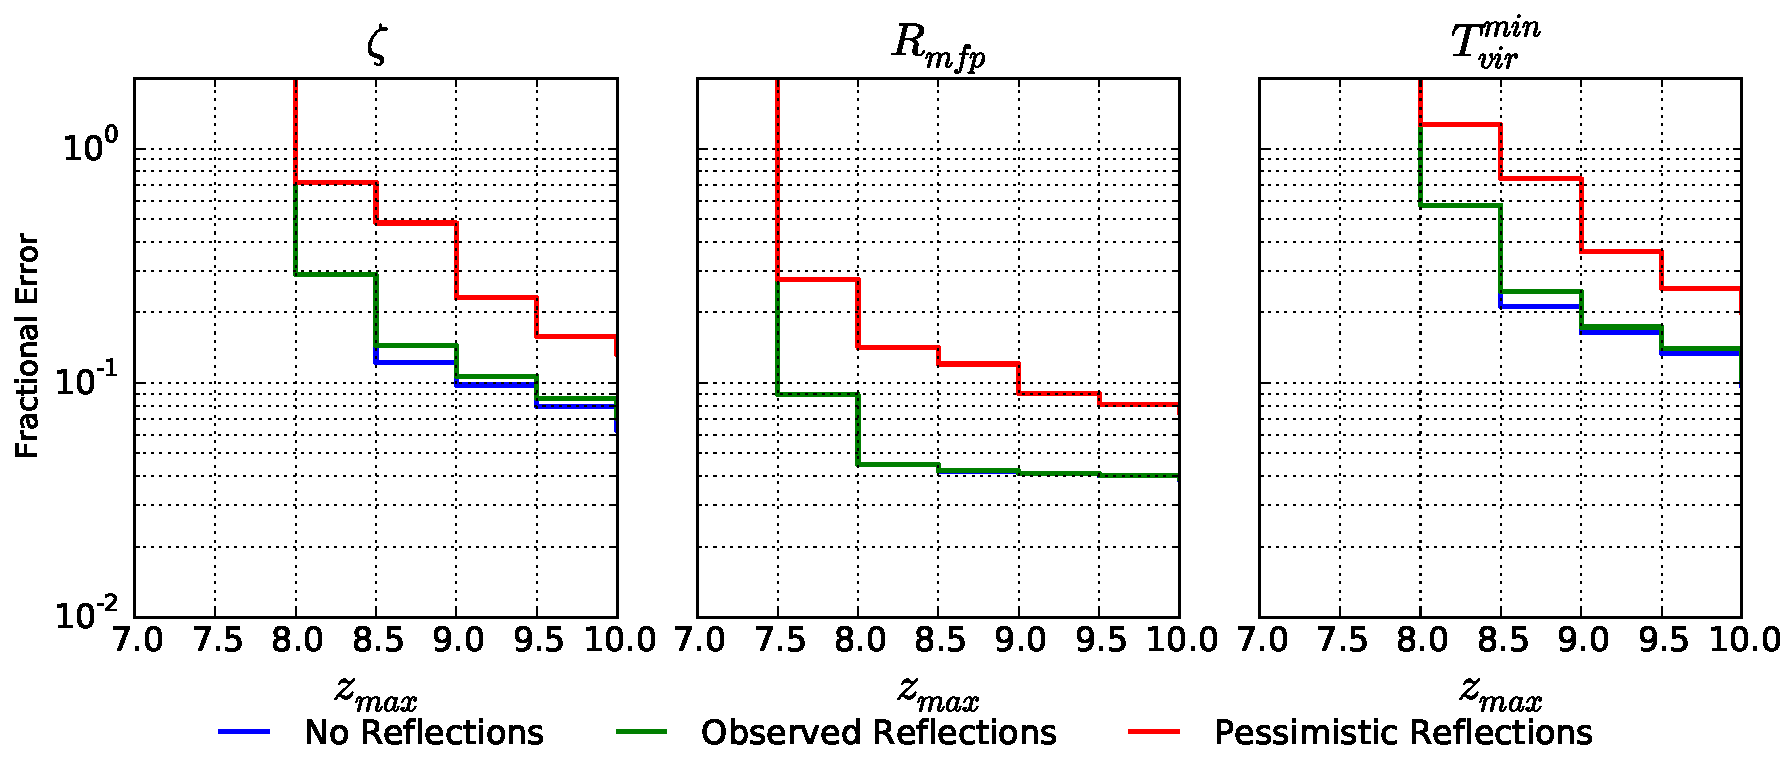
\includegraphics[width=\textwidth]{figures/sigmaVsZ_reionization_v2.pdf}
\caption{Fractional Errors on reionization and heating parameters as a function of maximal observed redshift out to the low end of HERA's initial observing band at $z=12$. The presence of strong reflections contained within a small subband at $z=8.5$ has a minimal impact on our overall constraints on reionization parameters. If these reflections are not localized they can lead to a factor of two loss in sensitivity to some parameters such as $T_\text{vir}^\text{min}$.}
\label{fig:Errors}
\end{figure*}

\begin{figure}[h!]
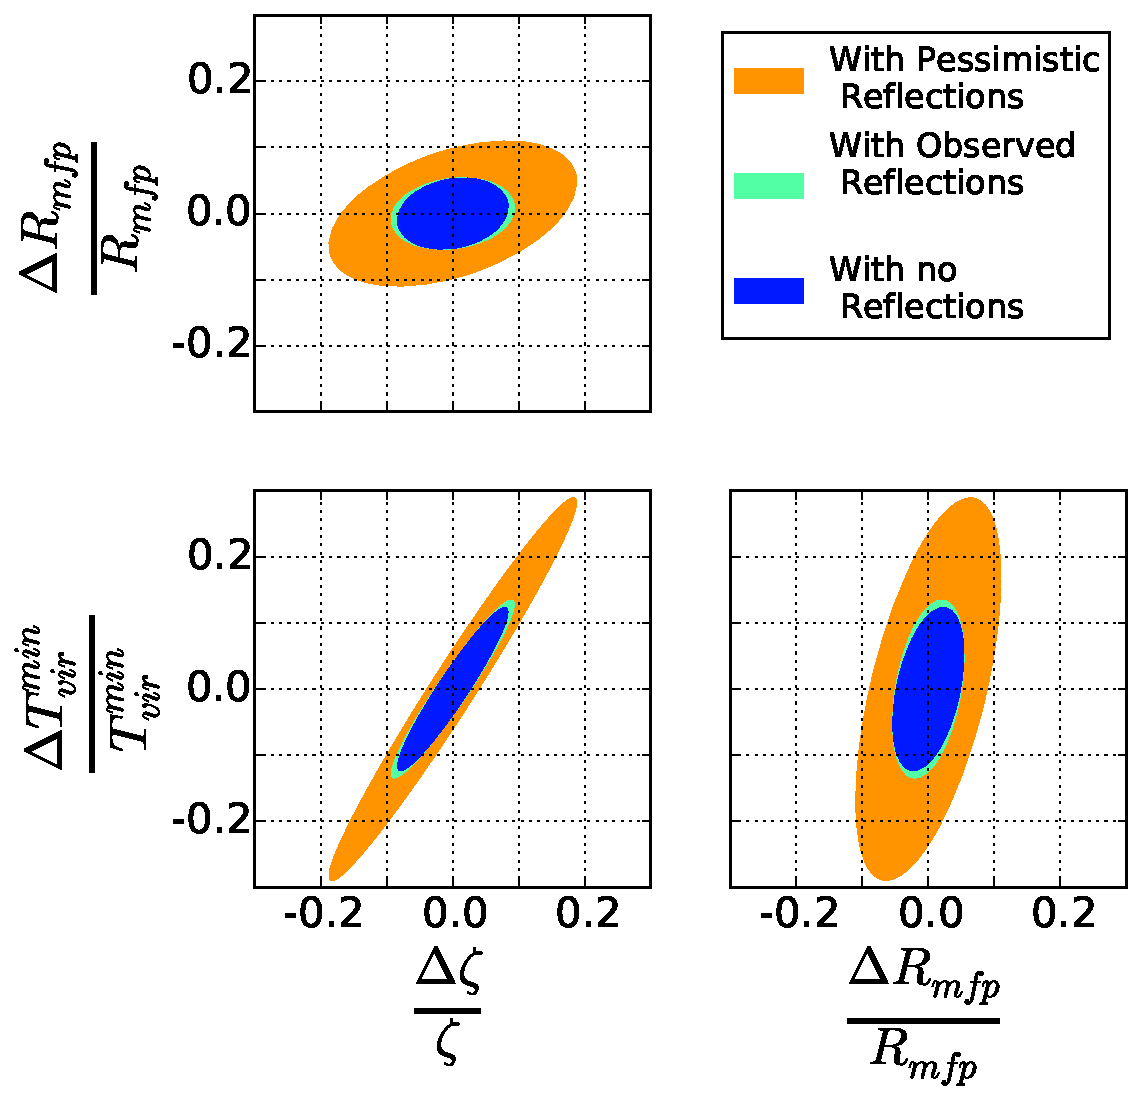
\includegraphics[width=.5\textwidth]{figures/reionization_triangle_compare_v2.pdf}
\caption{95\% confidence regions with and without reflections assuming that observations are taken over the redshifts between 7.5 and 10. The presence of the reflections leads to an increase in the major axes of these confidence regions by a factor of one to two.}
\label{fig:Confidence}
\end{figure}


We have seen in Fig.~\ref{fig:BothBaselines} that the simulated chromaticity of the dish leaks foregrounds beyond the horizon to varying degrees depending on the subband with the worst leakage occuring at $z=8.5$ centered at 150\,MHz in which foregrounds exceed the signal out to $\sim 380$\,ns which for a $14.6$\,m baseline is $\approx 330$\,ns beyond the horizon. At all other redshifts, the leakage due to beam chromaticity only extends to $\approx 250$\,ns beyond the horizon. To determine the potential impact of our observed beam chromaticity on HERA's ability to constrain the astrophysics of reionization, we consider three different scenarios for beam chromaticity that capture a range of possibilities allowed by our simulation. 


\begin{itemize}
\item {\bf Optimistic: The observed reflections are an artifact of the simulation.} It is possible that the long term reflections observed in the center of our gain are artifacts of our modeling and that effects such as dissipative effects due to unmodeled non-idealities in the geometry of the disk will allow reflected radio waves to be better absorbed or escape into space, suppressing these reflections. In our most optimistic scenario, we assume their absence in which case the foregrounds pass below the level of the signal at $240$\,ns beyond the horizon at all redshifts between $z=7$ and $10$, consistent with what is observed in the bands where the dish chromaticity is less severe or when it is not present at all. We do not consider the possibility that optimal inverse covariance weighting of the foregrounds  may actually decrease the minimal delays accessible to below the $250$\,ns above the horizon observed in our simulations. Hence, this scenario is actually somewhat conservative and certainly more pessimistic than the ones considered in \citep{Pober:2014,Greig:2015a,EwallWice:2015b}. 
 
\item {\bf Moderate: The Simulations accurately capture the chromaticity of the dish.} In this case, we assume that the reflections cause foregrounds to pass below the level of the signal at $250$\,ns except at redshift $8.5$ where they pass below the foregrounds at $350$\,ns. 


\item {\bf Pessimistic: The reflections are present in all sub-bands.} In this scenario, we assume that the spectral structure observed in the neighborhood of $150$\,MHz is present throughout the entire $100$-$200$\,MHz frequency range covered by HERA. While more pessimistic than anything we actually observe in our simulations, this scenario serves as a reasonable upper bound.
 
\end{itemize}
In Fig.~\ref{fig:Sensitivity}, we compare the level of $1\sigma$ thermal noise for our optimistic and moderate scenarios at $z=8.5$ to the amplitude of the 21\,cm signal. While the level of thermal noise monotonically increases with $k$, there is a small upturn at the smallest $k$ values due to an increase in sample variance caused by the knee like maximum in the 21\,cm power spectrum at $k \approx 0.1$\,$h$Mpc$^{-1}$ and the shrinking number of measurements within each 1d $k$-bin. Despite this upturn, the smallest $k$ modes are still the highest signal to noise measurements that HERA is expected to obtain, leading to a reduction in the maximal signal to noise ratio of $\approx 1.5$ and a reduction in the number of modes that the instrument is able to measure. 

Folding our calculations of thermal noise and the derivatives of $\Delta^2$ into equation~\ref{eq:Fisher} and inverting, we obtain the covariance matrix for model parameters from which we calculate $95\%$ confidence regions which we plot in Fig.~\ref{fig:Confidence}. The presence of reflections within a limited sub-band about $z=8.5$ leads to an almost neglible increase in the extent of our confidence intervals while the presence of the reflections across the entire band causes the length and width of our confidence ellipses to increase by a factor of $\approx 2$. The diagonal elements of our covariance gives us error bars on each parameter which we plot in Fig.~\ref{fig:Errors}. We see that similar to our confidence regions, the error bars on reionization parameters for our optimistic and moderate scenarios are nearly indestinguishable. In our worst case where reflections of a similar level as observed in the middle of our band are present everywhere, we see an increase in our error bars by a factor of $\approx 2$. 

The error bars on reionization parameters, even for our most optismtic model, are a factor of a few larger than the ``moderate" errors predicted in previous works using the Fisher Matrix such as \citet{Pober:2014}, \citet{EwallWice:2015a}, and \citet{Liu:2015a,Liu:2015b}. There are several reasons for this. Firstly, in our most optimistic scenario, we assumed that foregrounds cause the signal to be inaccessible below $250$\,ns beyond the edge of the wedge while in all previous works, a comoving $k$ of $k_\text{min}=0.1$\,$h$Mpc$^{-1}$, rather than a delay was used. In particular, this delay corresponds to a comoving $k\approx0.15$\,$h$Mpc$^{-1}$ at $z=8.5$, in significant excess of the values used in previous works. However, we do not consider the potential for inverse covariance techniques to further isolate foregrounds and potentially allowing us to work closer to the wedge than a naive Fourier transform. Because of this, our work is significantly more conservative than previous estimates. Secondly, previous studies assumed a fully illuminated HERA aperture, which for a $14$\,m dish predicts and effective area of $\approx155$\,m$^2$ at $150$\,MHz. Electromagnetic simulations and mapping of the primary beam of the HERA dish described in \citep{Neben:2015c} indicate are in good agreement that the effective area of the antenna element is actually $\approx 98$\,m$^2$ at $150$\,MHz which leads to an increase in the overall thermal noise levels by a factor of $\approx 1.5$. 

\section{Conclusions}
In this paper, we have formally described the impact of instrumental chromaticity on foreground contamination of the 21\,cm signal. We have also used simulations of electromagnetic waves incident from zenith on the primary antenna element on HERA to determine the extent to which reflections and other frequency dependent structure might leak foregrounds into the EoR window. The results of our simulations of the zenith gain of the instrument are broadly consistent with data obtained using reflectometry described in \citep{Patra:2015} and can be summarized in the following points. 
\begin{itemize}
\item The 14-m dish and inverted dipole feed configuration introduces reflections and, as a result, spectral structure, that is in excess of that observed in the antenna design for HERA's predecessor, PAPER. The dish design is intended to greatly increase array collecting area over PAPER without significantly raising the number of correlated elements while narrowing the angular field of view and suppressing the overall amplitude of foregrounds but we find that in achieving these ends, some degree of spectral smoothness has been sacrificed. Because foreground filtering in delay space cannot distinguish between signal and foregrounds, any regions of $k$-space contaminated by these reflections are effectively unusable in a 21\,cm measurement unless they can be modeled to high fidelity and removed. 

\item Fortunately, these reflections appear to be contained within the central $10$\,MHz of the HERA band, indicating a resonance that, in principle can be identified in the dish design and mitigated. It is also possible that the  non-ideal properties of an actual antenna will allow these reflections to escape the dish after a short time or be dissipated, rather than reflecting continually to long delays. Because estimates of the power spectrum are obtained from sub-intervals of $\approx10$\,MHz, the reflections that we have simulated will only impact a single redshift.

\item Simulating the impact of these reflections on foreground leakage using the foreground model described in \citet{Thyagarajan:2015c}, we find that the beam chromaticity extends foregrounds above the level of the cosmological signal to $\approx 350$\,ns beyond the horizon while without the reflections, foregrounds extend above the signal to $\approx 250$\,ns beyond the horizon. These observations are pessimistic in that no attempt to inversely weight the foregrounds by their covaranciances has been attempted. 

\item If the reflections are contained within a $10$\,MHz subband around $150$\,MHz, than the overall constraints that HERA will be able to place on the astrophysics of reionization are minimally impacted. If the reflections somehow contaminate the entire band, than our constraints on reionization parameters will suffer a factor of two increase in uncertainty but still remain on the order of $10$\%. 
\end{itemize}

\label{sec:Conclusion}
\bibliographystyle{apj}
\bibliography{DishSimulation_paper_v0}

\appendix
\section{The Effect of Reflections and Cross-Talk on Visibilities}\label{app:Reflections}
In this section, we investigate, formally, the impact of reflections of electromagnetic waves between antennas and within the signal chain of single antennas on foreground leakage in 21\,cm experiments. We start with the time varying electric field from a single source with location ${\bf \widehat{k}}$ on the sky, arriving at antenna $i$ with delay $\tau_i$ and antenna $j$ with delay $\tau_j$ with respect to the electric field at the origin which we denote as $s(t,{\bf \widehat{s}})$. We allow for two different types of reflections: First, we allow reflections within the analogue path of each $i^{th}$ antenna which we denote as $r_i(\tau,{\bf \widehat{s}})$. We also allow for single reflections between any $i-j$ antenna pair which we denote as $r_{ij}(\tau',{\bf \widehat{s}})$. Our choice of arbitrary $\tau'$, for now, allows for multi-path propogation between antennas, though we expect it to be dominated by the geometrical delay between the antenna pair. The electric field at antenna $i$ is given by
\begin{equation}
s_i(t,{\bf \widehat{s}}) = \int d \tau' r_i(\tau',{\bf \widehat{s}})s(t+\tau_i-\tau') + \sum_{j \ne i} \int d \tau' s(t + \tau_j - \tau_{ij}) r_{ij}(\tau',{\bf \widehat{s}})
\end{equation}  
In an FX correlator, the electric field is sampled, Fourier transformed, and cross multipled between antenna pairs to form visibilities. The Fourier transform step leaves us with 
\begin{equation}
\widetilde{s}_i(f,{\bf \widehat{s}}) = \widetilde{s}(f,{\bf \widehat{s}}) \left[ \int d \tau' r_i(\tau',{\bf \widehat{s}})e^{2 \pi i(\tau_i - \tau')f} + \sum_{j\ne i} \int d \tau' e^{2 \pi i(\tau_j - \tau_{ij})f} r_{ij}(\tau',{\bf \widehat{s}}) \right]
\end{equation}
Multiplying and averaging gives us the visibility for the single source we obtain
\begin{align}\label{eq:SingleSource}
v_{ij}'(f,{\bf \widehat{s}}) & = \langle \widetilde{s}_i(f,{\bf \widehat{k}}) \widetilde{s}_j(f,{\bf \widehat{s}}) \rangle_t \nonumber \\
&=d \Omega  I(f,{\bf \widehat{s}}) g_i(f) g_j^*(f) a_i(f,{\bf \widehat{s}})a_j^*(f,{\bf \widehat{s}}) e^{2 \pi i{\bf u_{ij}} \cdot {\bf \widehat{s}}} + d \Omega I(f,{\bf \widehat{s}}) \sum_{\ell \ne j} g_i(f)a_i(f,{\bf \widehat{s}}) C_{\ell j}^*(f,{\bf \widehat{s}}) e^{2 \pi i {\bf u_{\ell i} \cdot {\bf \widehat{s}}}} \nonumber \\ 
& + d \Omega I(f,{\bf \widehat{s}})\sum_{k \ne i} g_j^*(f) a_j^*(f) C_{ki}(f,{\bf \widehat{s}}) e^{2 \pi i {\bf u_{kj}\cdot {\bf \widehat{s}}}} + d \Omega I(f,{\bf \widehat{s}}) \sum_{k\ne i}\sum_{\ell \ne j} C_{ki}(f,{\bf \widehat{s}}) C_{j\ell}^*(f,{\bf \widehat{s}}) e^{2 \pi i {\bf u_{k\ell}}\cdot{\bf \widehat{s}}},
\end{align}
where $g_i(f) a_i(f,{\bf \widehat{s}}) = \int d \tau r_i(\tau,{\bf \widehat{s}}) e^{2 \pi i f \tau}$ is the effective direction dependent gain of the system which can be factored into a directoin dependent and direction independent function where $g_i(f)$ is the gain of the analogue signal chain after the radiation has been absorbed by the feed and $a_i(f,{\bf \widehat{s}})$ describes the chromatic electric field response of the antenna. The first term in equation~\ref{eq:SingleSource} is an effective visibility with self-reflections. The two cross terms and the last term involve the mixing of visibilities complementary too the $ij$ baseline and have the potential to introduce significant chromatic features since they potentially insert visibilities on much longer basline lengths. Assuming propogation along a single path directly between the antennas, we may write $C_{ik}(f,{\bf \widehat{s}})$ as 
\begin{equation}
C_{ki}(f,{\bf \widehat{s}}) = a_i(f,{\bf \widehat{s}}_{ki}) \frac{1}{r_{ik}}\left[\frac{d \sigma_k}{d \Omega}(f,{\bf \widehat{s}},{\bf \widehat{s}}_{ik})\right]^{1/2} e^{2 \pi i \tau_{ik} f}
\end{equation}
Where $r_{ik}$ is the distance between antennas $i$ and $k$, $d \sigma_k (f,{\bf \widehat{s}},{\bf \widehat{s}}_{ij})/ d \Omega $ is the cross-section of the antenna to scatter radiation from the ${\bf \widehat{s}}$ direction to the ${\bf \widehat{s}}_{ik}$ direction where ${\bf \widehat{s}}_{ik}$ is the unit vector in the direction between antenna $i$ and antenna $k$. Integrating over the primary beam, we obtain a full expression on the effect of the foregrounds. 
\begin{align}
V_{ij}' = \int d \Omega v_{ij}'(f,{\bf \widehat{s}}) &= g_i(f) g_j(f)^* \int d \Omega A_{ij}(f,{\bf \widehat{s}}) I(f,{\bf \widehat{s}})e^{2 \pi i f {\bf u_{ij}} \cdot {\bf \widehat{s}}} + g_i(f) \sum_{\ell \ne j} \int d \Omega  A_{i\ell j}(f,{\bf \widehat{s}}) I(f,{\bf \widehat{s}})e^{2 \pi i {\bf u_{\ell i} } \cdot {\bf \widehat{s}} } \nonumber \\ 
& + g_j^*(f) \sum_{k \ne i}  \int d \Omega A^*_{jki}(f,{\bf \widehat{s}}) I({\bf \widehat{s}},f) e^{2 \pi i {\bf u}_{kj} \cdot {\bf \widehat{s}} } + \sum_{k \ne i} \sum_{\ell \ne j}\int d \Omega A_{k i \ell j}(f,{\bf \widehat{s}}) I(f,{\bf \widehat{s}})e^{2 \pi i {\bf u}_{k\ell} \cdot {\bf \widehat{s}}}
\end{align}
which is essentially an ad-mixture of many baselines with different effective primary beams. We denote the effective primary beam of the $i,j$ antenna pair as $A_{ij}(f,{\bf \widehat{s}})=a_i(f,{\bf \widehat{s}})a_j^*(f,{\bf \widehat{s}})$, the effective beam from a single reflection correlated with a direct measurement as $A_{i \ell j} = a_i(f,{\bf \widehat{s}}) C^*_{\ell j}(f,{\bf \widehat{s}})$ and the correlation between entirely reflected terms as experiencing an effective primary beam of $A_{k i \ell j}=C_{ki}(f,{\bf \widehat{s}}) C^*_{j \ell}(f,{\bf \widehat{s}})$. In this paper, we focus on the reflection terms within a single antenna element. Hence, we ignore all but the first term for now. Any reflection terms occurring downstream of the conversion by the feed from electromagnetic radiation to voltage are lumped into $g_i(f)$ and reflections occurring within the antenna element enter into $a_i(f,{\bf \widehat{s}})$. While reflections within the analogue system are a potential source of contamination, HERA's post-feed analogue signal path is designed to keep all reflections under 35\,m, within the wedge. 

The focus of this paper and its companions is the reflection properties of the primary antenna element, so we will focus the rest of our discussion here on $a_i(f,{\bf \widehat{s}})$. The primary elements of our dish include a feed and backplane suspended over a fourteen meter dish. We assume a set of discrete reflections within the dish, which without loss of generality are assumed to have frequency independent reflection coefficients\footnote{If we allow each coefficient to be frequency dependent, we can expand each frequency dependent term in a Fourier series of frequency independent terms} hence 
\begin{equation}
a_i(f,{\bf \widehat{s}}) = \sum_{n} r_n({\bf \widehat{s}}) e^{2 \pi i  \tau_n f}
\end{equation}
Assuming all antennas are identical, we have
\begin{equation}
A_{ij}(f,{\bf \widehat{s}}) = \sum_m \sum_n r_n({\bf \widehat{s}}) r_m^*({\bf \widehat{s}}) e^{2 \pi i(\tau_n-\tau_m)f} = \sum_\alpha A_\alpha({\bf \widehat{s}}) e^{2 \pi i \tau_\alpha}
\end{equation}
where we have re-indexed $m$ and $n$ under a single greek index $\alpha$ in the second equality. The effect of internal reflections on a visibility is hence
\begin{equation}
V_{ij}'= \sum_\alpha \int d \Omega A_\alpha({\bf \widehat{s}}) e^{2 \pi i \tau_\alpha f} e^{2 \pi i {\bf b}_{ij} \cdot {\bf \widehat{s}}f/c} I(f,{\bf \widehat{s}})
\end{equation}
Taking the delay transform, one obtains
\begin{equation}
\widetilde{V}_{ij}'(\tau) = \sum_\alpha \widetilde{V}_{ij}^\alpha (\tau - \tau_\alpha)
\end{equation}
where 
\begin{equation}
\widetilde{V}^\alpha_{ij}(\tau) = \int d \tau e^{-2 \pi i f \tau} \int d \Omega A_\alpha({\bf \widehat{s}}) e^{2 \pi i {\bf b}_{ij} \cdot {\bf \widehat{s}} f/c} I(f,{\bf \widehat{s}})
\end{equation}
is the usual delay transform of \citet{Parsons:2012}. $\widetilde{V}_{ij}^alpha(\tau)$.
\end{document}